\documentclass[11pt]{article}

% ---------- Packages ----------
\usepackage[utf8]{inputenc}
\usepackage[T1]{fontenc}
\usepackage{amsmath,amssymb,amsfonts}
\usepackage{geometry}
\geometry{margin=1in}
\usepackage{microtype}
\usepackage{graphicx}
\usepackage{longtable}
\usepackage{array}
\usepackage{booktabs}
\usepackage{enumitem}
\usepackage[table]{xcolor}
\usepackage{titlesec}
\usepackage{caption}
\usepackage{tikz}
\usetikzlibrary{arrows.meta,positioning,shapes.geometric,shapes.symbols}
\usepackage{hyperref}

% ---------- Colours ----------
\definecolor{accent}{RGB}{0,64,128}
\definecolor{headerbg}{gray}{0.90}

% ---------- Heading styles ----------
\titleformat{\section}{\normalfont\Large\bfseries\color{accent}}{\thesection}{1em}{}[\color{accent!60}\titlerule]
\titlespacing*{\section}{0pt}{3.5ex plus 1ex minus .2ex}{2ex plus .2ex}
\titleformat{\subsection}{\normalfont\itshape\large}{}{0em}{}
\titlespacing*{\subsection}{0pt}{2.5ex plus 1ex minus .2ex}{1ex plus .2ex}

% ---------- Lists ----------
\setlist[description]{leftmargin=1.5em, style=nextline}
\setlist[itemize]{nosep, leftmargin=1.5em}
\setlist[enumerate]{nosep, leftmargin=1.5em}

% ---------- Tables ----------
\renewcommand{\arraystretch}{1.2}
\captionsetup{labelfont=bf, font=small}

% ---------- Typography ----------
\widowpenalty=10000
\clubpenalty=10000
\emergencystretch=2em
\setcounter{tocdepth}{1}

\hypersetup{
    colorlinks=true,
    linkcolor=accent,
    urlcolor=accent,
    citecolor=accent,
    pdftitle={SDR-Based Spectrum Monitoring System for FM Broadcast Compliance Assessment},
    bookmarksnumbered=true
}

% ---------- Custom column types for tables ----------
\newcolumntype{L}[1]{>{\raggedright\arraybackslash}p{#1}}
\newcolumntype{C}[1]{>{\centering\arraybackslash}p{#1}}

\title{SDR-Based Spectrum Monitoring System for FM Broadcast \\ Compliance Assessment}
\author{}
\date{}

\begin{document}

\begin{center}
    {\LARGE\bfseries SDR-Based Spectrum Monitoring System \\ for FM Broadcast Compliance Assessment\par}
    \vspace{0.6em}
    {\large Technical Specification \textendash{} \today\par}
\end{center}
\vspace{0.5em}
{\color{accent}\hrule height 1pt}
\vspace{0.8em}
\tableofcontents

\section*{Introduction}
\addcontentsline{toc}{section}{Introduction}

\subsection*{Purpose and Scope}

This document specifies the architecture, measurement framework, and processing algorithms for a Software-Defined Radio (SDR) based FM broadcast compliance monitoring system. It is intended for:

\begin{itemize}
    \item RF engineers designing and deploying sensor nodes;
    \item Regulatory bodies evaluating technical adequacy and metrological traceability;
    \item Software developers implementing DSP processing pipelines;
    \item System operators responsible for calibration, validation, and evidence archiving.
\end{itemize}

This document is primarily a framework and requirements specification. The framework addresses the complete monitoring chain with explicit treatment of calibration hierarchy, uncertainty propagation, node health, multi-node coordination, and audit-ready reporting.

\subsection*{Regulatory Context}

The system targets compliance assessment under the following regulatory and technical frameworks:

\begin{itemize}
    \item FCC Part 73 (United States): Technical standards for FM broadcast service, including carrier frequency tolerance, occupied bandwidth, and emission mask requirements;
    \item ANE Resoluci\'on 105 (Colombia): National regulatory provisions governing FM broadcast technical parameters;
    \item ITU-R BS.412: International technical standards for FM sound broadcasting;
    \item ITU-R BS.450-4: Transmission standards for FM sound broadcasting at VHF (signal model, maximum deviation, stereophonic multiplex);
    \item ITU-R SM.2152: Definitions of Software-Defined Radio (SDR), providing the terminology basis for the SDR architecture;
    \item ISO/IEC 17025: General requirements for the competence of testing and calibration laboratories, applicable to measurement traceability and uncertainty evaluation.
\end{itemize}

For each deployment, the applicable regulatory basis shall be explicitly identified in the system configuration, measurement procedure, and reporting policy. All reported measurands, decision outcomes, and compliance determinations shall be traceable to the governing rule set, the calibration state of the measurement chain, and the documented processing and decision procedure used to produce the result.\footnote{Throughout this document, the key words ``shall'', ``shall not'', ``should'', ``should not'', and ``may'' are to be interpreted as described in RFC 2119. Requirements denoted by ``shall'' are mandatory for compliance with this specification.}

\section{System-Level Requirements for SDR-Based Monitoring Architectures}

\begin{description}

\item[Reconfigurability and Flexibility] The SDR platform shall support changes in monitoring objectives, signal-processing parameters, and compliance algorithms without hardware redesign, consistent with the ITU-R SM.2152 definition of software-defined radio, in which RF operating parameters such as frequency range, modulation type, and output power are set or altered by software. Functions such as demodulation, channelization, thresholding, occupancy analysis, and report generation shall be implemented in software to permit controlled adaptation to evolving regulatory requirements, extension to adjacent bands, and integration of validated processing methods. Any software or firmware change affecting measurement outputs shall be documented, version-controlled, and revalidated.

\item[Cost and Deployability] The monitoring node shall be economically deployable at scale while preserving the performance required for regulatory use. Low-cost SDR hardware and embedded processing platforms may be used, provided they do not compromise frequency accuracy, calibration validity, or operational reliability. The final architecture shall be justified on the basis of both technical adequacy and total deployment cost.

\item[Remote Monitoring and Data Transport] The system shall support remote transmission of measurement metadata, system-health information, and authorized derived products to a centralized server through IP-based networks. The architecture shall support continuous or scheduled delivery, local buffering during link outages, and reliable upload upon reconnection. Data products, transport rates, retention policies, and latency constraints shall be defined according to the monitoring mission, legal requirements, and available network capacity.

\item[Cybersecurity and Access Control] Data in transit shall be protected using authenticated encryption, and stored records shall be protected according to the system security policy. Administrative and operator access shall be controlled through authenticated and authorized mechanisms. Audit logs shall record configuration changes, software updates, user actions, and remotely triggered monitoring operations.

\item[Multi-Channel Monitoring Capacity] The DSP pipeline shall support real-time demodulation and compliance analysis of multiple FM broadcast channels within the instantaneous observation bandwidth and tuning constraints of the SDR front-end and processing platform. The minimum sustained concurrent channel count shall be established through benchmarking on the deployment hardware. Validation shall document processor utilization, memory consumption, storage throughput, end-to-end latency, and the maximum sustainable channel count without sample loss or measurement degradation.

\item[Measurement Integrity, Calibration, and Traceability] The monitoring architecture shall preserve the metrological integrity of all reported measurands. The receive chain, including antenna, RF front-end, SDR, timing reference, and processing stages, shall support calibration, periodic verification, documented uncertainty, and reproducible performance across deployed nodes, in accordance with the metrological-traceability and equipment-calibration requirements of ISO/IEC 17025:2017 (clauses 6.5 and 6.4.6). All reported measurands, compliance decisions, alerts, and archived evidence shall be traceable to the acquisition record, receiver configuration, timing reference, calibration state, processing configuration, uncertainty characterization, and applicable regulatory rule. Any change affecting the measurement chain shall require revalidation of the corresponding calibration and reporting functions.

\end{description}

To support this requirement, the system shall implement a hierarchical calibration strategy with three tiers, aligned with the regulatory significance of the measurement.

\begin{description}

\item[Tier 1: Primary (Laboratory) Calibration] Each monitoring node shall undergo initial end-to-end calibration in a controlled laboratory environment, traceable to national or international standards. This calibration shall establish the absolute accuracy of the measurement reference plane, typically the antenna port, and shall characterize frequency response, power accuracy, linearity, and relevant environmental sensitivities. A unique calibration certificate and electronic calibration record shall be maintained for each node.

\item[Tier 2: Secondary (Field) Verification] Each node shall undergo periodic in situ verification to confirm that performance remains within acceptable limits relative to the primary calibration state. This procedure may use an internal reference source or a stable external signal. It need not re-establish absolute traceability, but shall provide a reliable check against predefined warning and alarm limits. Failure shall trigger a maintenance alert and suspend compliance use until resolved.

\item[Tier 3: Relative (Channel) Calibration] For measurements that do not require absolute power accuracy, a relative calibration across the observation bandwidth shall be maintained to control gain and phase distortion in spectral measurements. This calibration may be implemented through equalization filters, pilot-based methods, or passband characterization established during primary calibration.

\end{description}

\section{Functional Decomposition of the Monitoring System}

The architecture resulting from these design considerations is summarized in Figure~\ref{fig:architecture}, which identifies the principal hardware and software components and their interconnections.

\begin{description}

\item[RF Front-End (Hardware Layer)] The monitoring node employs a SDR receiver as the antenna-coupled RF front end for operation in the VHF-II broadcast band, spanning 87.5--108~MHz (the ITU Region 2 planning band), of which the regulated FM broadcast service band occupies 88--108~MHz. This stage captures incident RF energy, tunes the band of interest, and produces digitized complex baseband samples for downstream processing. A VHF-II antenna interfaces to the SDR input, and an LNA may be added when required to compensate for feedline loss or weak received signals. The suitability of this front end is governed by instantaneous bandwidth, dynamic range, frequency-reference accuracy and stability, noise figure, and gain configuration, since these parameters bound the fidelity of derived compliance measurands.

\item[Signal Acquisition and Digitization] The SDR streams raw complex baseband (I/Q) samples to the embedded host processor through a high-speed USB interface. These samples represent the instantaneous tuned observation bandwidth and permit simultaneous inspection of multiple contiguous FM broadcast channels within a single acquisition window, on the applicable 100~kHz (ANE channel plan) or 200~kHz (FCC channelization) raster, reducing the need for sequential retuning. The selected sample rate shall be validated on the target platform to ensure sustained operation without dropped samples, taking into account USB throughput, host buffering, and processing load.

\item[Software Processing Engine] The software processing engine implements the end-to-end DSP pipeline for FM broadcast compliance monitoring. Its functions may include spectrum estimation, channelization, carrier detection, demodulation, occupancy assessment, feature extraction, alarm generation, and compliance-metric evaluation. The primary output of this layer is not user-traffic recovery, but reported measurands, decision outcomes, and supporting evidence suitable for regulatory review.

\item[Data Management and Reporting Layer] Processed outputs shall be stored in a structured backend using time-stamped records and associated metadata, including frequency, site, station identifier, measurement type, and compliance status. This layer supports historical trend analysis, event review, audit-ready report generation, controlled remote access through an API and monitoring dashboard, and automated notifications when predefined thresholds are exceeded in accordance with the operational monitoring policy.

\end{description}

\begin{figure}[htbp]
\centering
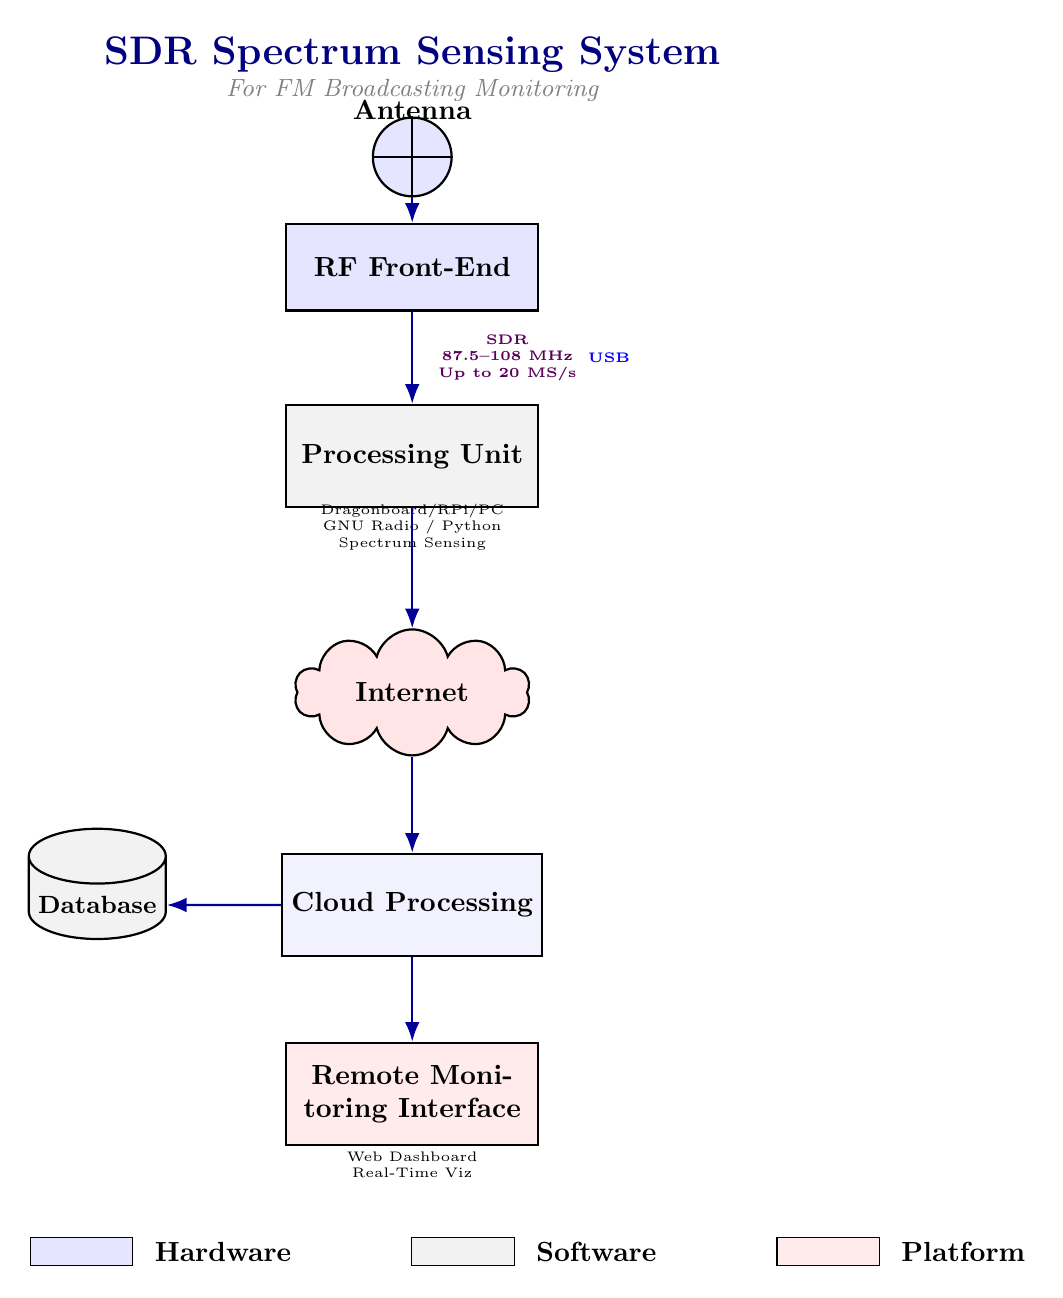
\begin{tikzpicture}[
    font=\small,
    box/.style={rectangle, draw=black, thick, minimum width=3.2cm, minimum height=1.1cm,
                align=center, font=\bfseries},
    hwbox/.style={box, fill=blue!10},
    swbox/.style={box, fill=black!5},
    platbox/.style={box, fill=red!8},
    cyl/.style={cylinder, shape border rotate=90, draw=black, thick, fill=black!5,
                minimum width=1.6cm, minimum height=1.4cm, aspect=0.4, align=center, font=\bfseries\small},
    cloudshape/.style={cloud, draw=black, thick, fill=red!10, aspect=2,
                        minimum width=3cm, minimum height=1.6cm, align=center},
    arr/.style={-{Latex[length=2.5mm]}, thick, blue!60!black},
    lbl/.style={font=\tiny\bfseries, align=center, text=violet!70!black}
]

% ---- Title ----
\node[align=center, blue!50!black] at (0,9.4) {\Large\bfseries SDR Spectrum Sensing System};
\node[align=center, gray] at (0,8.95) {\itshape For FM Broadcasting Monitoring};

% ---- Antenna ----
\node[circle, draw=black, thick, fill=blue!10, minimum size=1cm] (antenna) at (0,8.1) {};
\draw[thick] (antenna.north) -- ++(0,-1);
\draw[thick] (antenna.south) -- ++(0,1);
\draw[thick] (antenna.west) -- ++(1,0);
\draw[thick] (antenna.east) -- ++(-1,0);
\node[font=\bfseries] at (0,8.7) {Antenna};

% ---- RF Front-End ----
\node[hwbox] (rf) at (0,6.7) {RF Front-End};
\draw[arr] (antenna.south) -- (rf.north);

% ---- Processing Unit ----
\node[swbox, minimum height=1.3cm] (proc) at (0,4.3) {Processing Unit};
\draw[arr] (rf.south) -- (proc.north)
    node[midway, right, lbl, xshift=2mm] {SDR\\87.5--108 MHz\\Up to 20 MS/s};
\node[lbl, blue] at (2.5,5.55) {USB};
\node[align=center, font=\tiny] at (0,3.4) {Dragonboard/RPi/PC\\GNU Radio / Python\\Spectrum Sensing};

% ---- Internet cloud (between Processing Unit and Cloud Processing) ----
\node[cloudshape] (net) at (0,1.3) {};
\node[font=\bfseries] at (0,1.3) {Internet};
\draw[arr] (proc.south) -- (net.north);

% ---- Cloud Processing ----
\node[swbox, minimum height=1.3cm, fill=blue!5] (cloud) at (0,-1.4) {Cloud Processing};
\draw[arr] (net.south) -- (cloud.north);

% ---- Database (attached to Cloud Processing) ----
\node[cyl] (db) at (-4,-1.4) {Database};
\draw[arr] (cloud.west) -- (db.east);

% ---- Remote Monitoring Interface ----
\node[platbox, minimum height=1.3cm] (mon) at (0,-3.8) {Remote Moni-\\toring Interface};
\draw[arr] (cloud.south) -- (mon.north);
\node[align=center, font=\tiny] at (0,-4.7) {Web Dashboard\\Real-Time Viz};

% ---- Legend ----
\node[rectangle, draw=black, fill=blue!10, minimum width=1.3cm, minimum height=0.35cm] (leg1) at (-4.2,-5.8) {};
\node[right=0.15cm of leg1, font=\bfseries] (leg1txt) {Hardware};

\node[rectangle, draw=black, fill=black!5, minimum width=1.3cm, minimum height=0.35cm, right=1.4cm of leg1txt] (leg2) {};
\node[right=0.15cm of leg2, font=\bfseries] (leg2txt) {Software};

\node[rectangle, draw=black, fill=red!8, minimum width=1.3cm, minimum height=0.35cm, right=1.4cm of leg2txt] (leg3) {};
\node[right=0.15cm of leg3, font=\bfseries] {Platform};

\end{tikzpicture}
\caption{Core Architectural Components}
\label{fig:architecture}
\end{figure}

\section{FM Compliance Measurands and Traceability Requirements}

For SDR-based FM broadcast monitoring, a measurand is a defined physical or derived quantity reported by the monitoring system for regulatory assessment. The architecture shall distinguish between primary compliance measurands, which directly support conformance evaluation, and secondary observables, which provide diagnostic or evidentiary support but do not by themselves establish compliance.

\subsection*{Primary Compliance Measurands}

Primary compliance measurands are those used directly to assess technical conformity under the applicable regulatory framework. They may include:

\begin{itemize}
    \item carrier frequency or frequency offset relative to the assigned channel (carrier frequency error: $\pm 2$~kHz under the ANE FM technical plan and under 47 CFR \S73.1545(b) for stations above 10~W transmitter output power; $\pm 3$~kHz at 10~W or less);
    \item calibrated received power or spectral power at a defined reference plane within the observation bandwidth ($\pm 2.5$~dB);
    \item field strength, when supported by antenna-factor characterization and end-to-end calibration of the receive chain ($\pm 3.5$~dB);
    \item occupied bandwidth and related spectral-containment indicators;
    \item adjacent-channel leakage or out-of-band emission level;
    \item modulation-related quantities, including peak deviation and, where required, multiplex power;
    \item channel occupancy over time, including persistence metrics derived from a documented detection rule.
\end{itemize}

\subsection*{Secondary Observables}

Secondary observables support interpretation, diagnosis, and audit review. They shall not be treated as standalone compliance determinations unless explicitly required by the governing measurement procedure. They may include:

\begin{itemize}
    \item demodulated audio excerpts;
    \item baseband or multiplex spectrum snapshots;
    \item spectrograms and time-frequency visualizations;
    \item anomaly scores or classifier outputs produced by statistical or machine-learning methods.
\end{itemize}

\subsection*{Measurement Conditions, Metadata, and Traceability}

Each reported measurand shall be stored together with its measurement conditions and associated metadata, including observation bandwidth, center frequency, sample rate, receiver gain state, antenna configuration, reference plane, calibration state, calibration record identifier, site identifier, timestamp reference, and processing-software version. For derived quantities, the processing method, averaging interval, uncertainty characterization, decision rule, and applicable regulatory threshold shall also be recorded to support verification, reproducibility, inter-node comparison, and technical review.

Table~\ref{tab:measurands} defines the principal compliance measurands used by the SDR-based FM monitoring system. For each quantity, it specifies the operational definition, units, estimation method, calibration dependence, reporting cadence, and applicable compliance reference.

\begin{longtable}{L{2.4cm}L{3.6cm}L{1.5cm}L{4.0cm}L{2.9cm}}
\caption{Operational definition of principal FM compliance measurands. Here, $\beta\%$ occupied bandwidth denotes the minimum frequency interval containing $\beta\%$ of the total integrated mean emission power.}
\label{tab:measurands}\\
\toprule
\rowcolor{headerbg}
\textbf{Measurand (Symbol)} & \textbf{Definition} & \textbf{Units} & \textbf{Estimation method / Calibration dependency} & \textbf{Reporting interval / Compliance reference} \\
\midrule
\endfirsthead
\toprule
\rowcolor{headerbg}
\textbf{Measurand (Symbol)} & \textbf{Definition} & \textbf{Units} & \textbf{Estimation method / Calibration dependency} & \textbf{Reporting interval / Compliance reference} \\
\midrule
\endhead
\bottomrule
\endfoot

Carrier frequency error ($\Delta f_c$) &
Difference between the estimated channel center frequency and the assigned frequency of the monitored FM station. &
Hz &
Spectral peak, centroid, or model-based estimation referenced to the node frequency standard. Calibration dependency: High; depends on frequency-reference accuracy, offset calibration, and drift compensation ($^*$). &
Periodic and event-triggered. Assigned-frequency tolerance: ANE FM technical plan ($\pm 2$~kHz); 47 CFR \S73.1545(b) ($\pm 2000$~Hz above 10~W; $\pm 3000$~Hz at 10~W or less). \\

Calibrated received power ($P_{rx}(B)$) &
Power measured at a defined receiver reference plane over a stated bandwidth $B$ after gain-state and frequency-response correction. &
dBm or dB$\mu$V &
PSD estimation followed by integration over the defined analysis bandwidth after receiver calibration. Calibration dependency: High; requires gain calibration, front-end response correction, and a documented reference plane. &
Periodic. Site- or policy-specific threshold; suitable for compliance use only when the reference plane is defined. \\

Field strength ($E$) &
Electric field strength at the monitoring antenna location, inferred from the calibrated receive chain and antenna factor. &
dB$\mu$V/m &
Conversion from calibrated received level using antenna factor, cable loss, and front-end corrections. Calibration dependency: Very high; valid only when antenna factor and end-to-end chain calibration are available. &
Periodic. Applicable field-strength rule adopted by the jurisdiction (e.g., 47 CFR \S73.315: $\ge$70~dBu over the principal community; BS.412-9 Table~1 planning minima). \\

Occupied bandwidth ($B_{occ}$) &
Width of the frequency band containing a specified percentage of the total integrated mean emission power. &
kHz &
Direct $\beta\%$ occupied bandwidth measurement on the recorded spectrum. Calibration dependency: Moderate; depends on frequency-response flatness, RBW/FFT configuration, and interference control within the analysis span. &
Periodic. Spectral-containment rule: 47 CFR \S73.317(b) (mask compliance deems occupied bandwidth $\le$240~kHz); ANE FM technical plan limits stereo signals to 256~kHz. \\

Adjacent-channel / out-of-band emission level ($L_{adj}, L_{OOB}$) &
Emission level measured in adjacent-channel or out-of-band regions, reported either relative to the in-band reference level or at the calibrated receiver reference plane. &
dBc or dBm &
Spectral integration or peak-envelope evaluation in predefined offset bands relative to the assigned carrier. Calibration dependency: High; requires dynamic-range validation, front-end linearity, and spectral calibration. &
Periodic and event-triggered. Emission-mask rule adopted by the regulator (47 CFR \S73.317(c)--(d); ANE FM technical plan non-essential-emissions mask), evaluated for the stated offset region and reference level. \\

Peak deviation / multiplex-related indicator ($\Delta f_{max}$, $P_{MPX}$) &
Maximum instantaneous frequency deviation and, where required, a multiplex-related modulation quantity derived from the FM baseband or demodulated composite signal. &
kHz, dBr, or other adopted MPX metric &
FM demodulation followed by deviation estimation and multiplex-power measurement using the adopted method. Calibration dependency: High; depends on demodulator linearity, deviation calibration, and composite baseband conditioning. &
Windowed estimate with periodic summary. Deviation and multiplex-power limits (BS.450-4: maximum $\pm 75$~kHz; BS.412-9 \S2.5.1: 60~s multiplex-power criterion) under the adopted monitoring procedure. \\

Channel occupancy over time ($O_T$) &
Fraction of the observation interval during which the channel is declared occupied according to a documented detection rule. &
\% &
Threshold-, energy-, or feature-based detection over repeated observation windows with a defined revisit strategy. Calibration dependency: Moderate; depends on threshold calibration, noise-floor estimation, and decision logic. &
Rolling summary. Occupancy definition and decision rule established by the monitoring policy. \\

\end{longtable}

\vspace{-0.8\baselineskip}
\noindent\small $^*$Carrier-frequency error shall be reported as a compliance measurand only when the node frequency reference has been validated by a traceable calibration procedure or by an external disciplined reference.

\subsection*{Classification Framework}

The SDR monitoring system shall classify each measurand based on hardware-constrained measurement quality. This classification dictates permissible regulatory use and defines required validation, calibration, and uncertainty characterization.

The following capability classes are defined:

\begin{description}

\item[Compliance-Grade] The measurand may be used directly to support formal regulatory compliance determinations, provided that all calibration, validation, and uncertainty requirements specified in this document are satisfied. The hardware platform, processing implementation, and end-to-end measurement chain have been validated to meet the applicable regulatory tolerance and uncertainty limits.

\item[Screening-Grade] The measurand may be used for anomaly detection, event screening, situational awareness, or preliminary assessment, but it shall not be used as the sole basis for a formal non-compliance determination without corroboration from a compliance-grade measurement or independent validation. Screening-grade measurements may trigger alerts, operator review, or deployment of higher-capability instrumentation, but they do not by themselves constitute regulatory evidence.

\item[Unsupported] The measurand cannot be reliably estimated with the deployed hardware configuration and shall not be reported for either compliance or screening use. Attempting to measure an unsupported quantity may produce outputs that are numerically valid but metrologically meaningless or systematically biased beyond correction.

\item[Conditional Compliance-Grade] The measurand may reach compliance-grade status on this hardware platform, but only after all enumerated preconditions in the Enhancement column of Table~\ref{tab:capability} have been implemented, independently validated, and recorded in a calibration certificate. Prior to that validation, the measurand shall be treated as Screening-Grade for all regulatory purposes. The preconditions are mandatory, not recommended.\footnote{While the above standard classes exist for professional equipment, this ad hoc class is suitable for low-cost SDR boards with several limitations.}

\end{description}

\subsection*{Metadata Requirements for Capability-Dependent Reporting}

Every reported measurand shall include in its metadata record:

\begin{itemize}
    \item The capability class under which it was acquired (compliance-grade, screening-grade, conditional compliance-grade, unsupported),
    \item Hardware platform identifier and configuration (ADC resolution, gain state, reference source),
    \item Applicable calibration tier(s) and calibration record identifier,
    \item Measurement uncertainty or, for screening-grade results, an explicit uncertainty disclaimer,
    \item Any hardware augmentation applied (external GPSDO, LNA, filter),
    \item Software version and processing-method identifier.
\end{itemize}

Screening-grade measurands shall be flagged in all reports and databases as \texttt{FOR SCREENING ONLY} and shall not appear in formal compliance summaries without explicit override justification and independent validation.

\subsection*{Uncertainty Budget and Reporting}

All measurements intended for regulatory compliance use shall be accompanied by a documented uncertainty evaluation in accordance with the Guide to the Expression of Uncertainty in Measurement (GUM, JCGM 100:2008). The uncertainty budget shall account for all known sources of random and systematic error, shall be traceable to the calibration hierarchy defined above, and shall be reported alongside the measurand value in all compliance records and evidence archives.

Uncertainty Classification, the associated Uncertainty-Aware Compliance Decisions, and Periodic Re-Evaluation Requirements are detailed later in this document.

\section{Node-Level DSP Pipeline for FM Compliance Monitoring}

The compliance monitoring pipeline transforms raw complex baseband observations into reported measurands, decision outcomes, and supporting evidence. However, the technical rigor of such a pipeline implementation is often challenged by the hardware-software interface.

The principal processing stages are shown in Figure~\ref{fig:pipeline} and described below.

\begin{figure}[htbp]
\centering
\resizebox{\linewidth}{!}{%
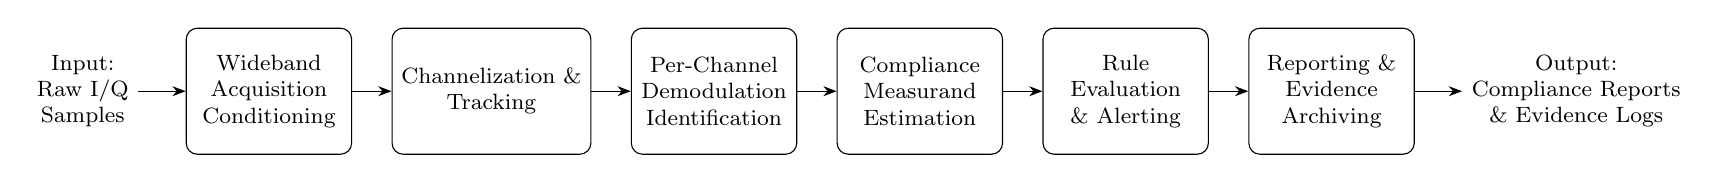
\begin{tikzpicture}[
    box/.style={draw, rectangle, minimum width=2.1cm, minimum height=1.6cm, align=center, rounded corners, font=\footnotesize},
    node distance=0.5cm
]
\node[box] (s1) {Wideband\\Acquisition\\Conditioning};
\node[box, right=of s1] (s2) {Channelization \&\\Tracking};
\node[box, right=of s2] (s3) {Per-Channel\\Demodulation\\Identification};
\node[box, right=of s3] (s4) {Compliance\\Measurand\\Estimation};
\node[box, right=of s4] (s5) {Rule\\Evaluation\\\& Alerting};
\node[box, right=of s5] (s6) {Reporting \&\\Evidence\\Archiving};

\node[left=0.6cm of s1, align=center, font=\footnotesize] (in) {Input:\\Raw I/Q\\Samples};
\node[right=0.6cm of s6, align=center, font=\footnotesize] (out) {Output:\\Compliance Reports\\\& Evidence Logs};

\draw[-Stealth] (in) -- (s1);
\draw[-Stealth] (s1) -- (s2);
\draw[-Stealth] (s2) -- (s3);
\draw[-Stealth] (s3) -- (s4);
\draw[-Stealth] (s4) -- (s5);
\draw[-Stealth] (s5) -- (s6);
\draw[-Stealth] (s6) -- (out);
\end{tikzpicture}%
}
\caption{Implemented SDR-based FM broadcast compliance monitoring pipeline. Raw I/Q samples are processed through six stages, from wideband acquisition and conditioning to reporting and evidence archiving, to enable automated regulatory assessment.}
\label{fig:pipeline}
\end{figure}

\subsection*{Wideband Acquisition \& Conditioning}

Raw I/Q samples are acquired from the SDR front end together with receiver-configuration and timing metadata. This stage establishes the wideband observation used by all downstream analyses.

Its principal functions are:
\begin{itemize}
    \item Hardware configuration: initialization of SDR operating parameters, including center frequency, sample rate, gain state, and front-end amplification settings;
    \item Sample streaming: transfer of raw complex baseband samples from the SDR device to the embedded host processor through the USB interface;
    \item Buffer management: temporary storage and flow control to reduce the risk of sample loss during sustained acquisition;
    \item Metadata association: tagging of captured data with timing, configuration, and calibration-state information;
    \item Signal conditioning: preliminary preparation of the wideband observation, including DC-offset mitigation, optional digital frequency translation, and other conditioning steps required before channelization and spectral analysis.
\end{itemize}

\subsection*{Channelization, Isolation \& Tracking}

The conditioned wideband observation is analyzed to detect active FM broadcast channels within the monitored span. Detected channels are isolated and tracked over time to support stable downstream measurement.

Its principal functions are:
\begin{itemize}
    \item Wideband spectral survey: estimation of spectral content over the monitored band to identify candidate FM emissions and their approximate center frequencies and occupied regions;
    \item Channel detection: application of detection criteria to distinguish active broadcast channels from noise, interference, or spurious responses;
    \item Channel isolation: extraction of individual FM channels through digital channelization, filtering, and frequency selection;
    \item Frequency tracking: monitoring of the spectral position of each detected channel to compensate for drift, tuning offsets, or minor carrier variations;
    \item Persistence assessment: evaluation of channel continuity and temporal presence to support occupancy estimation, event detection, and stable downstream demodulation.
\end{itemize}

\subsection*{Optional Per-Channel Demodulation \& Identification}

Each isolated FM channel is demodulated to recover the signal products required for modulation analysis. Auxiliary identification functions may be used to support station recognition, event attribution, or diagnostic interpretation, but they do not constitute primary compliance criteria.

Its principal functions are:
\begin{itemize}
    \item FM demodulation: conversion of each isolated RF channel into its corresponding baseband representation for subsequent compliance analysis;
    \item Composite baseband recovery: extraction of the FM multiplex signal components relevant to deviation analysis, pilot detection, stereo-related features, and other modulation-dependent measurements;
    \item Baseband conditioning: preparation of the recovered signal through filtering, normalization, and related operations required by the adopted estimation methods;
    \item Auxiliary station identification: use of identifying signal characteristics, such as spectral signatures, pilot structure, metadata cues, or program-dependent features, to support station recognition and event attribution;
    \item Secondary feature classification: optional classification of non-primary signal attributes for diagnostic interpretation, anomaly screening, or evidentiary support.
\end{itemize}

\subsection*{Compliance Measurand Estimation}

For each monitored channel, the system computes the operationally defined measurands required for regulatory assessment. Its main functions are:
\begin{itemize}
    \item Carrier-frequency estimation: determination of channel center frequency and its deviation relative to the assigned broadcast frequency, referenced to the adopted frequency standard and calibration state;
    \item Power-related estimation: computation of calibrated received power, spectral power, or other amplitude-related quantities at the defined reference plane, subject to the applicable gain and frequency-response corrections;
    \item Bandwidth and spectral-containment estimation: evaluation of occupied bandwidth and related spectral-containment indicators from the recorded spectrum using the adopted analysis bandwidth and decision rule;
    \item Adjacent- and out-of-band emission analysis: measurement of spectral leakage or emission level in adjacent-channel and out-of-band regions relative to the in-band reference level or other stated compliance reference;
    \item Modulation-related estimation: extraction of deviation-based and multiplex-related quantities from the demodulated baseband or composite signal;
    \item Occupancy estimation: determination of channel occupancy over time using the documented detection rule, observation window, and revisit strategy;
    \item Result association: association of each reported measurand with the relevant processing configuration, averaging interval, calibration state, and metadata.
\end{itemize}

\subsection*{Decision Logic \& Alerting}

The estimated measurands are compared against applicable regulatory limits, license conditions, or monitoring rules. When threshold exceedances or anomalous conditions are detected, the system generates alerts and records the supporting decision context.

Its principal functions are:
\begin{itemize}
    \item Compliance-rule matching: comparison of each estimated measurand against the applicable thresholds, license requirements, or monitoring criteria;
    \item Decision logic execution: application of the adopted decision rules to classify the observed channel state as compliant, non-compliant, uncertain, or requiring further review;
    \item Threshold exceedance detection: identification of events in which one or more measurands depart from their permitted range;
    \item Anomaly handling: processing of abnormal system or signal conditions that merit operator attention even when a formal violation is not established;
    \item Alert generation: creation of notifications, warning flags, or event markers for operator review;
    \item Decision-context recording: storage of supporting measurands, timestamps, processing parameters, rule set, and relevant metadata required to justify the alert or compliance decision.
\end{itemize}

The rule evaluation stage shall compare each estimated measurand $x$ against the applicable regulatory threshold $T$ using an explicitly defined decision rule that accounts for measurement uncertainty $U$. The decision logic depends on the regulatory framework, risk tolerance, and adopted compliance philosophy. Three supported decision frameworks are detailed later in this document.

\subsection*{Reporting \& Evidence Archiving}

The final stage stores reported results, selected signal products, and decision records in a structured backend for later retrieval, review, and audit.

Its principal functions are:
\begin{itemize}
    \item Measurement persistence: storage of reported measurands, decision outcomes, and associated metadata in a structured backend;
    \item Evidence preservation: retention of selected supporting artifacts, such as PSD estimates, spectrograms, demodulated excerpts, and event-linked channel records;
    \item Compliance reporting: generation of summaries, station-level assessment records, and historical trend outputs suitable for operational monitoring and formal review;
    \item Alert-log management: archival of alert histories, event markers, severity levels, and operator-facing notifications;
    \item Controlled access and retrieval: provision of structured mechanisms for querying, visualizing, and exporting stored results in accordance with the monitoring policy and access-control model.
\end{itemize}

The estimation background of the processing pipeline is specified for each Compliance Measurand in Section~\ref{sec:estimation}.

\section{Array-Level Coordination for Distributed Regulatory Monitoring}

In a distributed regulatory monitoring deployment, the sensor array shall be treated as a coordinated measurement system rather than as a collection of independent SDR nodes. Each node may acquire, preprocess, and estimate local measurands independently, but any array-level conclusion shall be formed only after the participating nodes have been brought into a common calibration, timing, reference, and health framework. This layer is necessary to ensure that multi-node conclusions remain technically comparable, metrologically defensible, and auditable under regulatory review.

\begin{description}

\item[Inter-node calibration] Each node shall retain its own primary, field, and relative calibration records, but the array shall additionally maintain an inter-node calibration model that quantifies residual differences between nodes for the measurands intended for joint use. This model shall include, at minimum, frequency-reference offset, gain bias, passband-shape deviation, timestamp offset, and any site-dependent correction needed to compare measurements across locations. Inter-node calibration shall be verified periodically using a shared reference signal, a transportable reference source, or a controlled over-the-air reference transmission. Array-level fusion shall use only nodes whose residual mismatch remains within predefined acceptance limits for the relevant measurand.

\item[Timing alignment] All nodes contributing to common event detection, occupancy estimation, or corroborated compliance decisions shall operate against a common time base traceable to UTC or another approved reference. Timestamp uncertainty, holdover behavior, synchronization-loss state, and timing-validation results shall be recorded in metadata. For array processing, observations shall be aligned to a documented common epoch and window definition, with explicit tolerance on allowable inter-node skew. If the required timing tolerance is exceeded, the affected node may continue local monitoring, but it shall be excluded from time-critical multi-node conclusions until synchronization is restored.

\item[Common reference distribution] The array shall distribute or derive a common frequency and time reference appropriate to the target measurement class. For carrier-frequency compliance, the use of a disciplined external reference shall be preferred where the node-local oscillator is otherwise insufficiently stable for the required tolerance. The reference architecture shall specify the reference source, distribution method, holdover strategy, fault detection, and the procedure followed when a node loses reference lock. Any measurement obtained during reference loss shall be flagged according to its impact on metrological validity and may be downgraded to screening-only use where required.

\item[Sensor health coordination] The array management layer shall continuously supervise node health using both hardware and measurement-quality indicators. These shall include SDR connectivity, sample-loss status, gain state, clipping, DC contamination, I/Q residuals, thermal alarms, storage availability, network reachability, calibration validity, synchronization state, and reference-lock state. Health supervision shall classify each node as at least one of the following: operational for compliance use, operational for screening only, degraded, or unavailable. Array-level conclusions shall only use nodes whose health state is compatible with the uncertainty and decision rule of the associated measurand.

\item[Cross-node consistency checks] When multiple nodes observe the same licensed emission or event, the system shall perform cross-node consistency analysis before issuing a fused regulatory conclusion. The consistency checks shall compare overlapping measurands after correcting for known site, antenna, and propagation differences. At minimum, the framework should evaluate consistency of carrier-frequency estimate, event time, occupancy declaration, and any jointly used spectral or modulation indicator. Persistent disagreement beyond the expected uncertainty budget shall trigger one of three outcomes: exclusion of the outlying node, classification of the event as uncertain, or escalation for operator review. Cross-node agreement shall strengthen confidence, but disagreement shall never be silently averaged away. This procedure is consistent with the validity-of-results monitoring concept of ISO/IEC 17025:2017, clause 7.7 (monitoring performance by comparison with results of other laboratories).

\item[Contribution of multiple nodes to one regulatory conclusion] The framework shall define a formal fusion rule for converting node-level results into an array-level conclusion. That rule shall specify:
\begin{enumerate}
    \item eligibility criteria for participating nodes;
    \item the measurands that may be fused and those that shall remain node-local;
    \item weighting factors based on calibration state, uncertainty, health, and geometry;
    \item the required corroboration level for declaring a non-compliance event; and
    \item how inconclusive or conflicting evidence is handled.
\end{enumerate}
For example, the array may adopt a rule in which a regulatory alert is issued only when at least two eligible nodes independently report the same exceedance within a defined time window and with compatible uncertainty bounds, while a single-node exceedance is retained as a provisional alert pending corroboration or review. The exact fusion rule shall depend on the measurand: carrier-frequency anomalies may be corroborated by agreement in calibrated frequency error, whereas occupancy or interference events may rely on synchronized temporal coincidence across nodes.

\item[Array-level traceability and evidence] Every fused decision shall preserve the full chain of evidence linking the array conclusion to the underlying node records. The archived record shall identify the participating nodes, their calibration states, synchronization states, health states, local uncertainties, fusion weights, consistency-check outcomes, and the decision-rule version used to form the final conclusion. This ensures that the array result remains auditable and can be reconstructed during technical or legal review.

\item[Degraded-mode operation] The framework shall explicitly distinguish between full array operation and degraded array operation. Loss of one node, loss of common reference, excessive timing skew, or calibration expiry shall not necessarily halt all monitoring, but it shall automatically restrict which measurement classes remain valid. In degraded mode, the system may continue screening, situational awareness, or evidence collection, while suspending array-level compliance determinations that depend on the missing capability.

\end{description}

\section{Baseline SDR Platform Assessment}

\subsection*{Measurement Capability, Platform Limitations, and Suitability}

A low-cost SDR device was selected for large-scale deployment on the basis of cost and reconfigurability. Its use as a primary sensor node entails a trade-off between cost-efficiency and metrological rigour that must be explicitly characterised before any compliance determination is made.

Regulatory emission masks (FCC Part 73 \S73.317(b)--(d); ANE Resoluci\'on 105, Anexo~2) impose stepped out-of-band attenuation: 25~dB at 120--240~kHz offset, 35~dB at 240--600~kHz, and the lesser of $43 + 10\log_{10} P$~(W) or 80~dB beyond 600~kHz under FCC rules (the ANE plan applies the same $43 + 10\log_{10} P$ expression beyond 600~kHz without the 80~dB cap), whereas the baseline SDR device's 8-bit ADC offers a theoretical dynamic range of only $\approx 50$~dB ($6.02 \times 8 + 1.76$~dB). In regulatory monitoring, the Effective Number of Bits (ENOB) is more critical than nominal bit depth: thermal noise, non-linearity, and input-power-dependent compression typically reduce practical resolution to $\approx 7$ bits ($\approx 42$~dB), with further degradation at the band edges of the instantaneous observation window. This limitation renders ACLR measurements and any measurand dependent on high dynamic range unreliable without external filtering and strict gain-staging.

To maintain metrological integrity, strict gain-staging protocols are required. Peak signal levels shall be maintained at least 6~dB below full scale to prevent clipping. In distributed deployments where the signal environment varies across nodes, this requires either manual gain profiling at each site or verified AGC with mandatory state logging. If AGC is employed, its state shall be recorded and timestamped for every sample block; measurements acquired without this metadata shall not be used for calibrated received power reporting and shall be flagged as invalid in the acquisition record.

The hardware's wideband nature introduces three DSP-level pathologies that affect different parts of the compliance measurand set:

\begin{description}

\item[DC spectral artifact] The LO leakage produces a narrowband spike at DC in the baseband spectrum. Offset tuning (setting $f_{LO} = f_{target} + f_{off}$, $f_{off} = f_s/4$) displaces the spike away from the measurement band and is the required mitigation. This increases acquisition complexity: precise mapping between the LO frequency, applied offset, and true RF frequency must be maintained and recorded in metadata.

\item[I/Q imbalance] Amplitude imbalance $g$ and phase error $\phi$ between the I and Q channels produce a mirror image of the desired signal at $-f_{offset}$ in the baseband spectrum. The correction applied in the preprocessing stage (a $2 \times 2$ widely-linear matrix with scalar $g$ and $\phi$) is frequency-independent. Across the instantaneous observation bandwidth, the SDR device's imbalance parameters are frequency-dependent; the scalar correction leaves a residual imbalance at frequencies remote from the calibration tone. Nodes operating with channel targets more than approximately 5~MHz from the calibration tone frequency shall re-estimate $g$ and $\phi$ at a tone within 500~kHz of the target channel, or shall bound the residual mirror power by measurement and record it as an uncertainty contributor. The corrected mirror power shall remain below $-40$~dBc after correction; results exceeding this threshold shall trigger the \texttt{IQ\_RESIDUAL} flag and shall not be used for occupied-bandwidth compliance estimation.

\item[Frequency-dependent noise floor] The receive chain exhibits a non-flat noise and gain profile across the observation bandwidth. A relative (Tier 3) calibration is required to characterise and correct this variation. The detection margin $\Delta_{det}$ used in Stage 4 channel detection is not a fixed absolute value; it shall be set as a site-calibrated offset above the locally verified noise floor, derived from the Tier 2 noise-floor verification required by the channel occupancy preconditions in Table~\ref{tab:capability}. A default value of 8~dB may be used only during initial commissioning prior to site verification; it shall not be used for compliance-grade or conditional-compliance-grade occupancy reporting.

\end{description}

Local-oscillator phase noise and the nominal $\pm 20$~ppm crystal reference accuracy constrain frequency stability. For carrier-frequency compliance, an external GPS-Disciplined Oscillator (GPSDO) providing a traceable 10~MHz reference is the required mitigation; validated post-hoc calibration alone is insufficient because it cannot correct for in-situ thermal drift between calibration intervals. Any measurement of carrier frequency error acquired without a locked GPSDO or equivalent disciplined reference shall be classified as screening-grade and flagged \texttt{UNCALIBRATED\_REFERENCE} regardless of any other configuration.

Additionally, the Stage 4 harmonic-rejection test is currently implemented as a placeholder and performs no rejection. Until this function is implemented and validated, nodes shall not be declared suitable for compliance-grade or conditional-compliance-grade use in deployment environments where intermodulation products from co-channel or adjacent FM stations may produce spurious candidates within the monitored span. Operators shall assess intermodulation risk at each site prior to compliance-use declaration by examining the wideband PSD for candidate energy at harmonic offsets from strong in-band carriers.

If any measurand class exceeds the validated hardware capability as defined in Table~\ref{tab:capability}, the node shall be declared unsuitable for that measurand and the corresponding output shall be suppressed or flagged \texttt{UNSUPPORTED} in all reports.

\subsection*{Upgrade Paths and Hybrid Architectures}

Deployments that require compliance-grade measurement of measurands currently classified as Screening-Grade or Unsupported in Table~\ref{tab:capability} shall implement one of the following strategies. The strategies differ in scope: Strategy~1 achieves compliance-grade coverage across all primary measurands; Strategy~2 achieves compliance-grade determination through array-level corroboration while retaining baseline SDR screening nodes; Strategy~3 elevates a defined subset of measurands to compliance-grade or Conditional Compliance-Grade on the baseline SDR platform through hardware augmentation and validation. In all cases, measurands classified as Conditional Compliance-Grade remain subject to the preconditions specified in Table~\ref{tab:capability}, regardless of which strategy is adopted.

\begin{enumerate}

\item \textbf{Hardware Upgrade.} Replace the baseline SDR device with a higher-performance SDR platform offering 12--16 bit ADC resolution, lower phase noise, improved SFDR, and a factory-calibrated or externally disciplined frequency reference. Candidate platforms include the Ettus Research USRP B200/B210 and the Airspy R2 or Airspy Mini (24--1800~MHz); equivalent instrumentation-grade receivers operating across the VHF-II band (87.5--108~MHz) are also acceptable. Full Tier 1 calibration of the replacement platform is mandatory prior to compliance-use declaration. Measurands classified as Conditional Compliance-Grade in Table~\ref{tab:capability} remain subject to their precondition lists even after a hardware upgrade.

\item \textbf{Hybrid Screening and Validation Architecture.} Deploy baseline SDR nodes for wide-area screening and event detection (Screening-Grade), supported by a smaller number of compliance-grade validation nodes equipped with higher-capability instrumentation at strategic locations. When a screening node triggers an alert, the event shall be corroborated by a compliance-grade node before any formal regulatory determination is issued. Corroboration shall follow the array-level fusion rules defined in Section~5, including eligibility criteria, inter-node calibration verification, timing alignment, and consistency checks. A single-node screening alert that cannot be corroborated within the defined time window and uncertainty bounds shall be retained as a provisional alert and escalated to operator review; it shall not constitute a standalone compliance determination.

\item \textbf{External Reference and Filtering Augmentation.} Retain the baseline SDR platform and augment each node with the following, all of which are mandatory for compliance-use declaration of the affected measurands:
\begin{itemize}
    \item External GPSDO providing a traceable 10~MHz reference and 1~PPS timing signal (required for carrier frequency error);
    \item External preselector or tunable bandpass filter to improve dynamic range for adjacent-channel measurements;
    \item Documented LNA with characterised gain and noise figure, inserted and calibrated as part of the Tier 1 receive-chain calibration;
    \item Automated AGC state logging and gain-step calibration, with per-block metadata recording;
    \item Implementation and validation of the Stage 4 harmonic rejection function prior to compliance-use declaration in any environment where intermodulation products from co-channel or adjacent FM stations may produce spurious candidates.
\end{itemize}
This approach elevates carrier frequency error and channel occupancy toward their respective target capability classes (Screening-Grade and Conditional Compliance-Grade), and may elevate occupied bandwidth to Conditional Compliance-Grade, subject to completion of all preconditions listed in Table~\ref{tab:capability} and documented uncertainty characterisation under the GUM framework. Field strength and adjacent-channel emission remain Unsupported under this strategy; compliance-grade assessment of these measurands requires Strategy~1.

\end{enumerate}

\subsection*{Capability Classification by Primary Measurand}

Table~\ref{tab:capability} summarises the baseline capability classification for each primary compliance measurand when the monitoring node is implemented using a baseline SDR receiver. The classification reflects the limitations imposed by the 8-bit ADC (effective $\approx 7$ bits, $\approx 42$~dB dynamic range), $\pm 20$~ppm uncalibrated frequency reference, front-end linearity, and noise floor characteristics described above.

The classification is a baseline: a node that has completed all mandatory preconditions listed for a Conditional Compliance-Grade measurand, and holds a current calibration certificate attesting to that completion, is reclassified to Compliance-Grade for that measurand only. In the absence of a valid certificate, the measurand shall revert to Screening-Grade regardless of any other system configuration.

For Unsupported measurands, the listed factors are hardware-imposed disqualifying limitations that cannot be resolved by calibration or software alone; the required platform capability is stated to guide upgrade decisions. For Screening-Grade measurands, the listed items are mandatory qualifications that must be satisfied before the measurand output is used for any monitoring purpose.

\begin{longtable}{L{3.2cm}L{2.2cm}L{8.6cm}}
\caption{Measurement Capability Matrix for the Baseline SDR--Based Monitoring Node. Classifications are baseline values; see paragraph above for reclassification conditions.}
\label{tab:capability}\\
\toprule
\rowcolor{headerbg}
\textbf{Measurand} & \textbf{Capability Class} & \textbf{Qualification, Preconditions, or Limiting Factors} \\
\midrule
\endfirsthead
\toprule
\rowcolor{headerbg}
\textbf{Measurand} & \textbf{Capability Class} & \textbf{Qualification, Preconditions, or Limiting Factors} \\
\midrule
\endhead
\bottomrule
\endfoot

Carrier Frequency Error & Screening &
External GPSDO required as the sole path to compliance-grade; post-hoc calibration alone is insufficient to correct in-situ thermal drift. Tier 1 calibration of frequency reference mandatory. Residual uncertainty shall be characterised and reported. Measurements acquired without a locked GPSDO shall be flagged \texttt{UNCALIBRATED\_REFERENCE} and treated as screening-grade regardless of other configuration. \\

Calibrated Received Power & Screening &
AGC state shall be recorded and timestamped for every sample block; measurements acquired without this metadata shall not be used for power reporting. Tier 1 and Tier 2 calibration of gain chain mandatory. Absolute power accuracy limited by gain quantisation (device-defined step sizes) and front-end uncertainty. Valid only when clipping is absent and gain state is recorded. \\

Field Strength & Unsupported &
Disqualifying limitations: (i) dynamic range of 35--45~dB is insufficient for weak-signal monitoring in the presence of strong co-channel or adjacent interference; (ii) no factory antenna-factor characterisation is available for the baseline SDR receive chain. Reclassification requires a platform with $\geq 12$-bit ADC, full end-to-end Tier 1 calibration including antenna factor, feedline loss, and environmental correction, and a validated site-specific antenna pattern. \\

Occupied Bandwidth & Conditional Compliance &
Mandatory preconditions --- all must be satisfied and attested by calibration certificate: (1)~FFT size, window function, and percentile method documented and version-controlled. (2)~Frequency-response flatness validated by Tier 3 calibration across the full analysis span, with residual ripple $< 0.5$~dB. (3)~RBW equivalent characterised and recorded in measurement metadata. (4)~Interference control within analysis span verified against a defined co-channel rejection criterion. (5)~I/Q imbalance correction residual verified $<-40$~dBc at the target channel frequency; results exceeding this threshold shall trigger \texttt{IQ\_RESIDUAL} and invalidate bandwidth estimates. (6)~Cross-validation against reference instrumentation (minimum one traceable signal generator sweep) completed and archived prior to first compliance-use deployment. \\

Adjacent-Channel / Out-of-Band Emission & Unsupported &
Disqualifying limitations: SFDR of 50--55~dBc is insufficient for the far-offset mask attenuation ($43 + 10\log_{10} P$ or 80~dB beyond 600~kHz); the gap cannot be closed by calibration. Reclassification requires an external preselector or SAW filter and a 14--16 bit ADC front-end; both are required, not optional. \\

Peak Deviation / Multiplex Power & Screening &
FM demodulator linearity and deviation calibration required. Multiplex-power estimation valid only when baseband conditioning (de-emphasis, pilot extraction) is validated against a reference modulation analyser. Pilot and RDS sub-carrier magnitudes shall be verified independently. \\

Channel Occupancy & Conditional Compliance &
Mandatory preconditions --- all must be satisfied and attested by calibration certificate, including site-calibrated detection threshold, statistical reporting model, and hysteresis/dwell parameters fixed under version control (see the Channel Occupancy requirements later in this document). \\

\end{longtable}

\subsection*{Theoretical vs. Practical Hardware Performance}

Table~\ref{tab:hardware} presents the theoretical versus practical hardware performance of the baseline SDR device for regulatory FM monitoring, together with the affected measurands.

\begin{longtable}{L{2.6cm}L{2.2cm}L{2.4cm}L{6.4cm}}
\caption{Theoretical vs. practical hardware performance of the baseline SDR device for regulatory FM monitoring. Affected measurands are identified to make the table actionable.}
\label{tab:hardware}\\
\toprule
\rowcolor{headerbg}
\textbf{Parameter} & \textbf{Theoretical} & \textbf{Practical (baseline SDR)} & \textbf{Impact on compliance (affected measurands)} \\
\midrule
\endfirsthead
\toprule
\rowcolor{headerbg}
\textbf{Parameter} & \textbf{Theoretical} & \textbf{Practical (baseline SDR)} & \textbf{Impact on compliance (affected measurands)} \\
\midrule
\endhead
\bottomrule
\endfoot

Dynamic range (ENOB-limited) & 49.9~dB (8-bit, $6.02 \times 8 + 1.76$) & 35--45~dB ($\approx 7$ bit effective) &
Insufficient for high-attenuation mask checks. Primary impact: ACLR, field strength. \\

SFDR & $\approx 48$~dBFS & 50--55~dBc &
Limited ability to distinguish weak spurs near strong carriers. Primary impact: ACLR, occupied bandwidth near band edges. Theoretical SFDR is expressed in dBFS (relative to full scale); practical SFDR is expressed in dBc (relative to a carrier tone). These are not directly comparable: a strong in-band carrier raises the apparent SFDR in dBc while the absolute spurious floor in dBm remains constrained by the 8-bit dynamic range. The dBFS figure governs compliance headroom calculations. \\

I/Q imbalance (scalar correction residual) & 0~dB mirror rejection (ideal) & $<-40$~dBc within $\pm 5$~MHz of cal.\ tone; degrades at band edges &
Mirror images bias spectral estimates and generate false candidates. Primary impact: carrier frequency estimation, occupied bandwidth. Frequency-dependent; re-calibration required per site channel. \\

LO phase noise & $<-100$~dBc/Hz at 10~kHz offset (ideal) & $-80$ to $-85$~dBc/Hz at 10~kHz offset (stock crystal oscillator) &
Broadens spectral estimates and raises close-in noise floor. Primary impact: carrier frequency error, occupied bandwidth edge interpolation. Mitigated by GPSDO with low-phase-noise 10~MHz reference. \\

Sampling rate (sustained) & Up to 20~Msps & Reliable at 10--16~Msps &
Limits instantaneous observation bandwidth for multi-channel survey. Primary impact: wideband acquisition coverage, multi-channel occupancy. \\

Frequency reference accuracy & N/A (XO-dependent) & $\pm 20$~ppm (stock crystal oscillator) &
$\pm 2$~kHz absolute error at 100~MHz; exceeds carrier-frequency compliance tolerance without GPSDO. Primary impact: carrier frequency error. \\

\end{longtable}

\noindent\small\textit{Sources: Dynamic range and SFDR values are based on the empirical characterisation of the baseline SDR device and on the following representative RF front-end and ADC datasheets: the Analog Devices (Maxim) MAX2837 direct-conversion RF transceiver (94~dB receive gain-control range); the Analog Devices (Maxim) MAX5865 dual 8-bit ADC front end (48.4~dB SINAD, 40~Msps class); the Realtek RTL2832U DVB-T demodulator with integrated 8-bit ADC (28.8~MHz reference crystal, $\pm$100~ppm class oscillator); the Rafael Micro R820T2 silicon tuner (24--1766~MHz); the Mirics MSI001 tuner (25~MHz--1.75~GHz); the Analog Devices AD9361/AD9363 agile transceivers with 12-bit ADCs (USRP B200/B210, ADALM-PLUTO); and the Lime Microsystems LMS7002M transceiver with 12-bit ADC (LimeSDR). Values for the 8-bit class are empirical baseline characterisations; values for the 12--16-bit classes are indicative datasheet figures. Phase noise figures are indicative; site measurement is recommended for compliance-critical deployments.}

\section{Reference Requirements for Full Compliance-Grade Deployments}

The following requirements apply to each measurand when compliance-grade or Conditional Compliance-Grade reporting is sought. Requirements for measurands classified as Unsupported on the baseline SDR platform (field strength, ACLR) are scoped to upgraded or augmented platforms as defined in the Upgrade Paths section; they do not imply that these measurands are achievable on the unaugmented baseline SDR device. All requirements are in addition to, not in substitution for, the preconditions listed in Table~\ref{tab:capability}.

\subsection*{Carrier Frequency Error and Stability}

\begin{itemize}
    \item \textbf{Reference clock traceability.} The SDR master clock shall be disciplined by a GPS-Disciplined Oscillator (GPSDO) or equivalent traceable reference providing a fractional frequency accuracy of $\pm 1 \times 10^{-9}$ or better. An external Rubidium oscillator is acceptable only when it is itself GPS-steered or carries a current calibration certificate traceable to a national frequency standard; a free-running Rubidium standard does not satisfy this requirement.
    \item \textbf{Estimation algorithm.} Carrier centre frequency shall be estimated using the Stage 5 pipeline specified later in this document (parabolic interpolation primary, power centroid and edge midpoint as supporting estimators). The power-weighted centroid may be used as the primary estimator only when the peak-parabolic method is flagged invalid by the Stage 5 validity logic.
    \item \textbf{Guard-band decision logic.} The Guard-Band rule (\eqref{eq:guardband}) shall be applied using the carrier-frequency tolerance applicable to the jurisdiction: $\pm 2000$~Hz ($>10$~W) / $\pm 3000$~Hz ($\le 10$~W) per 47 CFR \S73.1545(b), or $\pm 2$~kHz under the ANE FM technical plan. If $|f_{cal} - f_{target}| + U \leq T$, the result is compliant; if $|f_{cal} - f_{target}| - U > T$, non-compliant; otherwise uncertain and subject to the escalation procedure in Table~\ref{tab:decision-rules}.
    \item \textbf{Uncertainty-driven escalation.} As specified in Table~\ref{tab:decision-rules}, results in the uncertain zone shall trigger a repeated measurement cycle with $4\times$ extended averaging. If the result remains uncertain after three attempts, it shall be logged as \texttt{UNRESOLVED} and escalated to operator review.
    \item \textbf{Reference drift monitoring.} The GPSDO lock state and 1~PPS timing validity shall be recorded continuously. Any measurement acquired during a GPSDO unlock event shall be flagged \texttt{UNCALIBRATED\_REFERENCE} and classified as screening-grade. Temperature of the SDR front-end shall be logged as a diagnostic field; if the node operates without a disciplined reference (e.g., during holdover), the estimated frequency drift based on the TCXO drift profile shall be recorded as an additional Type B uncertainty contribution.
\end{itemize}

\subsection*{Calibrated Received Power}

\begin{itemize}
    \item \textbf{Reference plane traceability.} The receive chain shall undergo Tier 1 laboratory calibration establishing absolute gain accuracy at the defined reference plane (antenna port or SDR input bulkhead). Tier 2 field verification shall confirm that the node has not drifted beyond acceptable limits relative to the Tier 1 state; Tier 2 alone does not establish absolute traceability.
    \item \textbf{Shared-risk decision logic.} Expanded uncertainty $U$ ($k=2$) shall be computed in real time. Values falling within the $U$-interval of the applicable ERP or received-power limit shall be flagged for verification using a calibrated mobile unit or a compliance-grade co-located node, per Table~\ref{tab:decision-rules}.
    \item \textbf{Integration method.} Calibrated received power shall be computed as the RMS-weighted PSD integral over the defined analysis bandwidth $B$ (nominally 200~kHz under FCC channelization; 100~kHz under the ANE channel plan), after gain-state and frequency-response correction.
\end{itemize}

\subsection*{Field Strength (upgraded or augmented platforms only)}

\begin{itemize}
    \item \textbf{Scope.} Field strength is classified Unsupported on the baseline SDR platform. The following requirements apply only to platforms satisfying the reclassification criteria stated in Table~\ref{tab:capability} (Field Strength row).
    \item \textbf{Antenna factor application.} Frequency-dependent antenna factors (AF) shall be applied to convert calibrated terminal power to field strength in dB$\mu$V/m. The AF table shall be derived from a Tier 1 antenna calibration and shall cover the full operating bandwidth at the deployment site.
    \item \textbf{Reference plane.} The field-strength reference plane is the antenna terminals. All feedline losses and connector corrections shall be characterised and applied as part of the Tier 1 calibration.
\end{itemize}

\subsection*{Occupied Bandwidth}

\begin{itemize}
    \item \textbf{Windowing.} Blackman-Harris windowing shall be used for all occupied bandwidth measurements, consistent with the Stage 3 spectral estimation pipeline. Flat-top windowing shall not be used; its non-zero passband ripple introduces systematic bias in the power integration used for the $\beta\%$ boundary determination.
    \item \textbf{RBW correction.} Normalised compensation for the equivalent noise bandwidth (ENBW) of the analysis window shall be applied before the $\beta\%$ power boundary is computed.
    \item \textbf{Adaptive resolution.} If the $\beta\%$ (99\%) boundary falls within 5~kHz of the regulatory mask limit, the system shall increase the FFT size to achieve finer bin resolution. Any change to the FFT size shall be logged in the measurement metadata and treated as a processing configuration change subject to version control, consistent with the Conditional Compliance precondition (1) in Table~\ref{tab:capability}.
    \item \textbf{I/Q residual gate.} Before reporting an occupied bandwidth result, the system shall verify that the \texttt{IQ\_RESIDUAL} flag is not set. Results acquired when the corrected mirror power exceeds $-40$~dBc shall be invalidated per Table~\ref{tab:capability} precondition (5).
\end{itemize}

\subsection*{Adjacent-Channel and Out-of-Band Emission (upgraded platforms only)}

\begin{itemize}
    \item \textbf{Scope.} ACLR is classified Unsupported on the baseline SDR platform. The following requirements apply only to platforms satisfying the reclassification criteria stated in Table~\ref{tab:capability} (ACLR row).
    \item \textbf{SFDR margin gate.} Before any ACLR measurement is reported, the system shall verify that the platform's in-situ SFDR exceeds the applicable regulatory mask limit by at least 15~dB. If this condition is not met, the measurement shall be suppressed and flagged \texttt{UNSUPPORTED}.
    \item \textbf{Integration bandwidth.} The integration window shall be defined as 200~kHz (FCC channelization) or 100~kHz (ANE channel plan) centred on the adjacent or alternate channel carrier. For Colombian deployments, the applicable adjacent-channel threshold is the ANE protection ratio (25~dB at $\pm 100$~kHz; 7~dB at $\pm 200$~kHz for station classes A/B/C/D).
    \item \textbf{Uncertain results.} Uncertain ACLR results shall not support a non-compliance determination. Escalation shall follow the array-level coordination procedure in Section~5 using a higher-dynamic-range validation node where available.
\end{itemize}

\subsection*{Peak Deviation and Multiplex Power}

\begin{itemize}
    \item \textbf{Demodulation bandwidth.} FM demodulation shall use a minimum IF bandwidth of 400~kHz to capture high-order sidebands. This is an internal engineering requirement of this specification; ITU-R BS.412 does not prescribe a receiver IF bandwidth.
    \item \textbf{MPX power reference.} Integration of the multiplex signal power shall be reported in dBr relative to the 0~dBr reference level, defined as the power of the composite MPX signal at 75~kHz peak deviation of a 1~kHz sine tone, with the 19~kHz stereo pilot present at its nominal level. This is an adopted procedure definition of this specification for reporting purposes; it is distinct from the multiplex-power criterion of ITU-R BS.412 \S2.5.1, which limits the power of the complete multiplex signal integrated over any 60~s interval to that of a single tone causing $\pm 19$~kHz peak deviation. Both definitions shall be recorded in the measurement procedure.
    \item \textbf{Sub-carrier verification.} The 19~kHz pilot tone and 57~kHz RDS sub-carrier shall be independently verified in magnitude. Results shall be reported relative to the main carrier level and stored as supporting evidence.
\end{itemize}

\subsection*{Channel Occupancy}

\begin{itemize}
    \item \textbf{Detection threshold.} The occupancy threshold shall be a site-calibrated offset above the locally verified noise floor, derived from the Tier 2 noise-floor verification required by Table~\ref{tab:capability} precondition (2). A fixed default offset shall not be used for Conditional Compliance-Grade reporting.
    \item \textbf{Statistical reporting.} Occupancy shall be reported as the fraction of observation windows in which the channel is declared occupied under the documented detection rule, together with a confidence interval derived from the characterised false-alarm and missed-detection probabilities. The reporting model shall be consistent with the statistical probability framework required by Table~\ref{tab:capability} precondition (3).
    \item \textbf{Hysteresis and dwell.} Temporal hysteresis shall be applied to prevent false occupancy triggers from intermittent burst signals. The hysteresis parameters shall be fixed in the version-controlled processing configuration per Table~\ref{tab:capability} precondition (4).
\end{itemize}

\section{Estimation Pipeline of Measurands}
\label{sec:estimation}

\subsection*{Reference Carrier-Frequency Estimation Procedure}

The processing pipeline is specified for estimating the carrier centre frequency of an FM broadcast signal from complex baseband samples acquired with an SDR receiver. The implementation is organised as six sequential stages. The pipeline is explicitly designed to retain intermediate quantities so that spectral estimates, candidate selection, carrier estimates, and confidence scores remain auditable and can be reinterpreted if calibration metadata are updated.

\subsubsection*{Stage 1: Acquisition Configuration}

The acquisition stage constructs a validated hardware configuration for one SDR capture session. In the notebook implementation, the receiver is configured with
\begin{equation}
f_{LO} = f_{target} + f_{off}, \qquad f_{off} = \frac{f_s}{4},
\end{equation}
so the observed FM channel is offset from the DC bin by one quarter of the sample rate. The configuration validator additionally requires
\begin{equation}
|f_{off}| \geq 300~\text{kHz}, \qquad |f_{off}| + 150~\text{kHz} < \frac{f_s}{2},
\end{equation}
so that the target FM allocation remains well separated from the DC region and inside the usable complex baseband span.

The user-facing SDR receive controls are:
\begin{itemize}
    \item RF amplifier state (internal front-end amplifier gain $G_{RF}$),
    \item IF gain in the device's native steps over its IF gain range,
    \item baseband gain in the device's native steps over its baseband gain range.
\end{itemize}

For compatibility with legacy drivers, alternate gain-control identifiers may be accepted and mapped to the IF and baseband gain stages respectively. The configuration records $f_{target}, f_{off}, f_{LO}, f_s$, together with the individual gain settings and the total receiver gain
\begin{equation}
G_{RX} = G_{RF} + G_{IF} + G_{BB},
\end{equation}
where $G_{RF}$ is the front-end amplifier gain specified by the device datasheet, taken as zero when the RF amplifier is disabled.

A warning is emitted when the total gain exceeds the notebook warning level of 32~dB, but clipping prevention is not enforced analytically at this stage.

During capture, the SDR device is configured in the sequence sample-rate $\rightarrow$ frequency $\rightarrow$ gain chain. A short tuning settling pause is inserted after setting the LO. Raw interleaved I/Q samples in the device's native format are collected and converted to normalized complex baseband as
\begin{equation}
x[n] = \frac{I[n] + jQ[n]}{2^{b-1}},
\label{eq:iq-normalization}
\end{equation}
where $b$ is the ADC resolution in bits and $2^{b-1}$ normalizes the signed full-scale range, and a warm-up segment of 131{,}072 complex samples is discarded before the final retained block is formed. Clipping is detected directly from the raw ADC stream by checking whether any sample equals a full-scale code, and this boolean clipping outcome is propagated to later stages.

SDR devices deliver raw I/Q samples in a device-specific numeric format that shall be recorded in the acquisition metadata. The commonly encountered formats, in the SoapySDR/GNU Radio nomenclature (a leading letter for the number type --- \texttt{C} complex, \texttt{F} floating point, \texttt{S} signed integer, \texttt{U} unsigned integer --- followed by the bit width of each I and Q component), are:

\begin{itemize}
    \item \texttt{CF32} --- complex float32 (8~bytes per sample): the DSP-native representation and de facto standard for stored IQ captures (the \texttt{.cfile} convention); no re-scaling is required and full dynamic range is preserved, at the cost of the highest transport and storage bandwidth;
    \item \texttt{CS16} --- complex int16 (4~bytes per sample): the workhorse for receivers with 12--16-bit ADCs; only the lower 12~bits are typically meaningful, and the valid bits may be left- or right-justified within the 16-bit word, so justification and byte order shall be recorded in metadata;
    \item \texttt{CS12} --- complex int12 (3~bytes per sample): packed 12-bit signed format used by several modern front ends to halve the wire bandwidth relative to \texttt{CS16};
    \item \texttt{CS8} --- complex int8 (2~bytes per sample): signed 8-bit format of 8-bit-ADC devices; halves transport bandwidth relative to \texttt{CS16} at the cost of coarse quantisation ($\approx 42$~dB dynamic range);
    \item \texttt{CU8} --- complex uint8 (2~bytes per sample): unsigned 8-bit format centred at mid-scale (code 127.5); the host shall re-centre the samples before DSP, and any residual DC bias is a property of the capture, not a defect of the format;
    \item \texttt{CS4} --- complex int4 (1~byte per sample): extreme-bandwidth-compressed signed format, occasionally used to sustain very wide observation spans over constrained links.
\end{itemize}

Samples are conventionally interleaved (I and Q components contiguous within each sample); planar and block-interleaved arrangements also occur and shall be identified in metadata. Conversion to the normalized complex representation of Eq.~\eqref{eq:iq-normalization} shall divide signed integer samples by the full-scale value $2^{b-1}$; unsigned formats (e.g., \texttt{CU8}) shall first be re-centred by subtracting the mid-scale code $2^{b-1}$. The reverse conversion shall clamp before truncation so that a hot sample cannot wrap around the integer range into a spurious value. The sample format, byte order, bit justification, and scale factor shall be version-controlled fields of the acquisition record.

\subsubsection*{Stage 2: Preprocessing}

The preprocessing stage operates on the retained complex baseband sequence and performs three sub-stages in fixed order: DC-spike mitigation, I/Q imbalance correction, and relative noise-floor estimation.

\paragraph{2a. DC-spike mitigation.} The notebook removes residual DC contamination by processing the signal in non-overlapping FFT blocks of length $N_{DC} = 4096$ by default. For each complete block, the spectrum is FFT-shifted, a symmetric guard region centred on the DC bin is identified, and the guarded samples are replaced by interpolated amplitude and phase derived from the adjacent non-guard context bins. With guard width $N_{guard} = 5$ and interpolation context $N_{ctx} = 4$, the guarded frequency span recorded in metadata is
\begin{equation}
W_{DC} = \frac{(2 N_{guard} + 1) f_s}{N_{DC}}.
\end{equation}
The implementation stores the mean pre-correction DC-bin power across the processed blocks as a diagnostic field. Any trailing remainder shorter than one FFT block is passed through unchanged.

\paragraph{2b. I/Q imbalance correction.} The corrected complex sequence is then passed through a $2 \times 2$ widely-linear correction matrix derived from the current \texttt{IQCalibration} object:
\begin{equation}
\tilde{x}[n] = C\, x[n], \qquad C = \begin{pmatrix} 1 & 0 \\ -\sin\phi & \cos\phi / g \end{pmatrix},
\end{equation}
where $g$ is the amplitude-imbalance factor and $\phi$ is the phase error in radians. The notebook also provides an estimate \texttt{iq\_calibration()} helper that estimates $g$ and $\phi$ from a reference tone, but the correction stage itself simply applies the supplied calibration.

Mirror-rejection diagnostics are computed only when an explicit evaluation tone offset is supplied. In that case the notebook measures mirror power before and after correction, reports the suppression in dB, and raises an I/Q residual flag when the corrected mirror remains above the notebook threshold of $-40$~dBc. When no diagnostic tone is supplied, mirror-power metrics are stored as NaN and no residual flag is asserted.

\paragraph{2c. Relative noise-floor estimation.} The final preprocessing sub-stage estimates a relative, pre-calibration noise baseline. The corrected sequence is partitioned into up to $K = 16$ complete, non-overlapping frames of length $N_{noise} = 4096$ by default. Each frame is windowed by a Blackman--Harris window normalized to unit RMS and transformed to the frequency domain. The frame power spectra $\{P_m(k)\}$ are accumulated, and the provisional baseline is formed from the per-bin percentile, with default percentile $p = 10$:
\begin{equation}
N_{prov}(k) = \text{percentile}_{10}\{P_m(k)\}_{m=1}^{K}.
\end{equation}

The notebook then protects the baseline against signal occupancy. It forms the mean spectrum across the same frames, converts both the provisional percentile baseline and the mean spectrum to dB, and marks as occupied any bins where the mean exceeds the provisional baseline by more than 6~dB. That occupied mask is dilated by 12 bins on each side, the masked baseline is linearly interpolated across the remaining unmasked bins, and the result is smoothed by a reflected moving-average filter of width 33 bins. If the protected mask would leave fewer than 10\% of bins unmasked, the notebook falls back to a smoothed version of the provisional baseline instead of interpolating through the mask.

The Stage 2 output therefore contains:
\begin{itemize}
    \item the DC-corrected and I/Q-corrected sample stream,
    \item the inclusive DC guard-band width,
    \item I/Q imbalance diagnostics,
    \item a relative frequency-dependent noise-floor estimate \texttt{noise\_floor\_relative\_db},
\end{itemize}
not yet a calibrated dBm/Hz baseline.

\subsubsection*{Stage 3: Spectral Estimation}

Stage 3 computes the calibrated wideband power spectral density used by the downstream detector and carrier estimator. The implementation requires
\begin{equation}
N_{FFT} \geq 8192, \quad N_{FFT} \text{ power-of-two}, \quad M \geq 4
\end{equation}
complete non-overlapping averaging frames. The default configuration is $N_{FFT} = 8192$, $M = 16$, and a Blackman--Harris analysis window. A boxcar window is explicitly rejected because the notebook treats its sidelobe suppression as inadequate for FM monitoring.

For each complete frame $m$, the PSD estimate is computed as
\begin{equation}
\hat{P}_m(k) = \frac{\left| \sum_{n=0}^{N_{FFT}-1} x_m[n]\, w[n]\, e^{-j2\pi k n / N_{FFT}} \right|^2}{f_s \sum_{n=0}^{N_{FFT}-1} |w[n]|^2},
\end{equation}
and Welch averaging yields
\begin{equation}
\hat{P}(k) = \frac{1}{M} \sum_{m=1}^{M} \hat{P}_m(k).
\end{equation}

The resulting average is first represented in dBFS/Hz, then converted to dBm/Hz by the scalar gain-calibration term
\begin{equation}
C_{gain} = (-10~\text{dBm}) - G_{RX} + L_{cable} - G_{ant},
\end{equation}
with the antenna term applied only when antenna correction is explicitly enabled. An optional per-bin frequency-response correction vector may also be applied when its length matches the FFT size.

The Stage 3 frequency axis is constructed as
\begin{equation}
f_k = f_{baseband,k} + f_{LO} - f_{off},
\end{equation}
so the Stage 1 tuning offset is already removed at this point. This is the frequency axis used by both Stage 4 and Stage 5.

The Stage 2 relative noise floor is then resampled from the Stage 2 FFT grid to the Stage 3 FFT grid by frequency interpolation. The calibrated Stage 3 noise floor is formed by adding both the Stage 3 scalar gain correction and the Stage 2 density offset
\begin{equation}
-10 \log_{10}(f_s N_{noise}),
\end{equation}
yielding the stored field \texttt{noise\_floor\_calibrated\_dbm\_hz}. The notebook also retains the resampled relative baseline separately as \texttt{noise\_floor\_relative\_db}. Shape and finiteness checks are applied to both arrays before Stage 3 returns.

\subsubsection*{Stage 4: Channel Candidate Detection}

Stage 4 does not search for isolated spectral lines. Instead, it detects occupied above-threshold regions in the calibrated PSD. A smoothed baseline threshold is formed from the calibrated noise floor:
\begin{equation}
T(k) = N_{cal}(k) + \Delta_{det},
\end{equation}
with default detection margin
\begin{equation}
\Delta_{det} = 8~\text{dB},
\end{equation}
and allowed bounds 6 to 20~dB. The threshold itself is smoothed by a reflected moving-average filter of width 9 bins.

The occupied-mask rule is
\begin{equation}
\hat{P}_{cal}(k) > T(k).
\end{equation}
Short gaps in that mask are closed when their width does not exceed the equivalent of 15~kHz. Regions shorter than the equivalent of 40~kHz are discarded.

For each surviving region $[k_s, k_e]$, the notebook computes:
\begin{itemize}
    \item peak bin and peak power inside the region;
    \item median calibrated noise floor over the region;
    \item region SNR as peak power minus regional median noise floor;
    \item raw occupied bandwidth $W_{occ} = f[k_e] - f[k_s]$;
    \item edge midpoint $f_{edge} = \frac{1}{2}\left(f[k_s] + f[k_e]\right)$;
    \item power centroid obtained from the positive linear-power excess above the calibrated noise floor across the region;
    \item shoulder power, defined as the maximum PSD in the left or right outer shoulder windows extending up to $\pm 400$~kHz beyond the region;
    \item region prominence $\Pi = P_{peak} - P_{shoulder}$.
\end{itemize}

The Stage 4 candidate centre frequency stored in the candidate object is the edge midpoint, not the peak-bin frequency and not the centroid. A bandwidth-out-of-range flag is raised when
\begin{equation}
W_{occ} \notin [40~\text{kHz}, 400~\text{kHz}].
\end{equation}

A candidate is considered a valid carrier only when it is not marked as an artifact, is not in DC proximity, is not width-rejected, and has
\begin{equation}
\Pi \geq 10~\text{dB}.
\end{equation}

The notebook includes three artefact checks:

\begin{enumerate}
\item \textbf{DC proximity:} in the currently executed run \texttt{stage4(...)} code path, the default argument \texttt{dc\_guard\_band\_hz} is 30~kHz, and the implemented flag test is
\begin{equation}
|f - f_{target}| < 2 \times 30~\text{kHz}.
\end{equation}
Hence, in the executed integration path, DC proximity is effectively tested within 60~kHz of the target frequency, not from a Stage 2-derived $W_{DC}$ expression.

\item \textbf{Mirror-image test:} in the current executed run \texttt{stage4(...)} code path, candidate pairs are compared around the reflection axis
\begin{equation}
f_{refl} = f_{target}.
\end{equation}
A candidate is marked as a mirror only when its paired reflected candidate lies within 5~kHz of the expected mirror location, differs in peak power by at least 6~dB, and has sufficiently similar bandwidth (minimum width ratio 0.5).

\item \textbf{Harmonic test:} harmonic flagging is present only as a placeholder and currently performs no rejection.
\end{enumerate}

Each candidate is ranked by the notebook score
\begin{equation}
S = 0.45\, S_{prox} + 0.25\, S_{snr} + 0.20\, S_{width} + 0.10\, S_{prom},
\end{equation}
where
\begin{equation}
S_{prox} = \exp\left(-\left(\frac{f_c - f_{target}}{150~\text{kHz}}\right)^2\right),
\end{equation}
\begin{equation}
S_{snr} = \text{clip}\left(\frac{SNR}{25}, 0, 1\right), \qquad
S_{width} = \begin{cases} 1, & W_{occ} \in [100, 250]~\text{kHz}, \\ 0, & \text{otherwise}, \end{cases}
\end{equation}
and
\begin{equation}
S_{prom} = \text{clip}\left(\frac{\Pi}{20~\text{dB}}, 0, 1\right).
\end{equation}

Candidates closer than 100~kHz are deduplicated by keeping the higher-scored candidate. The return list is ordered as all valid carriers in descending score, followed by invalid candidates in descending score, and is truncated to at most 8 entries.

\subsubsection*{Stage 5: Carrier-Frequency Estimation}

Stage 5 estimates the carrier frequency from the primary valid candidate returned by Stage 4 unless a different candidate is explicitly supplied.

\paragraph{Primary estimator: peak-centric parabolic interpolation.}
The primary estimator is a three-point parabolic interpolation around the peak bin inside the selected occupied region. The notebook accepts the Stage 4 threshold array only for shape validation and API compatibility; it is not used as a Stage 5 peak-validity gate. The validity logic is purely geometric and local.

Let $k^\star$ be the maximum-PSD bin inside the region. The estimator first requires that $k^\star$ is not on the global spectral boundary and that the peak is a local maximum in the dB domain:
\begin{equation}
y_0 \geq y_{-1}, \qquad y_0 \geq y_{+1},
\end{equation}
with local prominence
\begin{equation}
y_0 - \max(y_{-1}, y_{+1}) \geq 0.5~\text{dB}.
\end{equation}

The quadratic refinement is then carried out in linear power:
\begin{equation}
p_{-1} = 10^{y_{-1}/10}, \quad p_0 = 10^{y_0/10}, \quad p_{+1} = 10^{y_{+1}/10},
\end{equation}
\begin{equation}
d = p_{-1} - 2 p_0 + p_{+1}, \qquad \delta = \frac{1}{2} \frac{p_{-1} - p_{+1}}{d}.
\end{equation}

The curvature must be finite, non-degenerate, and concave ($d < 0$). The raw sub-bin offset must satisfy
\begin{equation}
|\delta| \leq 1.
\end{equation}
If so, it is clipped conservatively into $\delta \in [-0.5, +0.5]$ before the refined frequency is reported:
\begin{equation}
\hat{f}_{peak} = f[k^\star] + \delta \, \Delta f_{bin}.
\end{equation}
If any of the above checks fails, the peak-parabolic method is marked invalid and Stage 5 falls back to a supporting estimator.

\paragraph{Supporting estimators.}
Two supporting estimators are always computed on the calibrated spectral arrays:
\begin{itemize}
    \item \textbf{Edge midpoint:} Stage 5 recomputes the left and right threshold crossings using the calibrated PSD and the calibrated Stage 4 threshold, linearly interpolates both crossings, and reports the midpoint frequency and interpolated edge bandwidth.
    \item \textbf{Power centroid:} Stage 5 computes a power centroid using the positive linear-power excess above the calibrated noise floor within the selected region.
\end{itemize}

\paragraph{Optional phase-domain refinement.}
The notebook preserves API switches for MUSIC and Pisarenko refinement but intentionally leaves phase-domain refinement disabled in the compliance-tuned Stage 5 path. The corresponding return field is therefore \texttt{None}.

\paragraph{WBFM-aware repeatability diagnostic.}
Legacy per-frame instantaneous frequency statistics are intentionally disabled in the current notebook because they are not physically meaningful for WBFM carrier-centre estimation. The fields \texttt{frame\_frequency\_estimates\_hz}, \texttt{frame\_std\_hz}, \texttt{frame\_mean\_hz}, and \texttt{frame\_inconsistency\_flag} are retained for compatibility but are set to
\begin{equation}
[\,], \quad 0, \quad \hat{f}_{primary\ fallback}, \quad \text{False},
\end{equation}
respectively, where $\hat{f}_{primary\ fallback}$ equals the peak-parabolic estimate when that estimate is valid, and otherwise equals the centroid estimate.

Instead, repeatability is measured across repeated averaged PSD estimates built from non-overlapping blocks of the Stage 3 frame spectra. The block count defaults to 4, limited by however many frame spectra are available. Within each block, the stored per-frame PSDs are converted from dB to linear power, averaged, converted back to dB, and re-estimated by the same Stage 5 method cascade: peak-parabolic $\rightarrow$ centroid $\rightarrow$ edge midpoint $\rightarrow$ fallback frequency. The resulting list $\{\hat{f}_{block,i}\}$ yields
\begin{equation}
\sigma_{block} = \text{std}\{\hat{f}_{block,i}\}, \qquad \mu_{block} = \text{mean}\{\hat{f}_{block,i}\}.
\end{equation}
A block-repeatability warning flag is raised when
\begin{equation}
\sigma_{block} > 1000~\text{Hz}.
\end{equation}
To ensure consistency with the stored Stage 3 frame spectra, the block repeatability estimator converts the calibrated Stage 3 noise floor and threshold back to the frame-relative domain by subtracting the Stage 3 scalar gain correction before applying the repeated-estimation cascade.

\paragraph{Final estimator selection.}
The notebook selects the final raw estimate as follows:
\begin{enumerate}
    \item use the peak-parabolic estimate if valid;
    \item otherwise use the centroid if finite;
    \item otherwise use the edge midpoint.
\end{enumerate}
A fallback flag and a fallback-reason string are emitted whenever the peak-parabolic estimate is invalid.

\paragraph{Frequency correction and deviation.}
The final calibrated estimate is
\begin{equation}
\hat{f}_{cal} = \hat{f}_{raw} + \varepsilon_{cal},
\end{equation}
where $\varepsilon_{cal}$ is the residual frequency-calibration correction supplied through \texttt{FrequencyCalibration}. No additional offset-tuning subtraction is applied in Stage 5 because the Stage 3 frequency axis has already been corrected for $f_{off}$.

The reported carrier deviation from the assigned frequency is
\begin{equation}
\Delta f = \hat{f}_{cal} - f_{target}.
\end{equation}

\paragraph{Uncertainty estimate.}
The Stage 5 residual-frequency uncertainty is a conservative maximum of:
\begin{itemize}
    \item a minimum interpolation residual equal to 5\% of the FFT bin spacing,
    \item the supplied calibration uncertainty,
    \item the block-repeatability standard deviation,
    \item pairwise disagreement terms between the available Stage 5 methods.
\end{itemize}
Formally, the notebook returns
\begin{equation}
u_f = \max\left(0.05\, \Delta f_{bin},\; u_{cal},\; \sigma_{block},\; |\hat{f}_{peak} - \hat{f}_{cent}|,\; |\hat{f}_{peak} - \hat{f}_{edge}|,\; |\hat{f}_{edge} - \hat{f}_{cent}|\right),
\end{equation}
with the peak-related terms included only when the peak-parabolic estimate is valid.

\subsubsection*{Stage 6: Confidence Scoring and Result Assembly}

The notebook computes a composite confidence scalar $C \in [0, 1]$ from six normalized sub-scores:
\begin{equation}
C = 0.25\, c_{agree} + 0.25\, c_{block} + 0.15\, c_{geom} + 0.15\, c_{region} + 0.10\, c_{margin} + 0.10\, c_{cal}.
\end{equation}

The six sub-scores are defined exactly as follows.

\paragraph{Agreement score $c_{agree}$.}
The notebook computes the method spread as the range of the finite values among $\hat{f}_{peak}, \hat{f}_{cent}, \hat{f}_{edge}$, and then sets
\begin{equation}
c_{agree} = \exp\left(-\left(\frac{\Delta f_{spread}}{1500~\text{Hz}}\right)^2\right).
\end{equation}

\paragraph{Block-repeatability score $c_{block}$.}
Using the Stage 5 block-repeatability standard deviation,
\begin{equation}
c_{block} = \exp\left(-\left(\frac{\sigma_{block}}{500~\text{Hz}}\right)^2\right).
\end{equation}

\paragraph{Peak-geometry score $c_{geom}$.}
This score combines the local parabolic-peak prominence and the absolute sub-bin offset:
\begin{equation}
c_{geom} = \text{clip}\left(\frac{\Pi_{local}}{2~\text{dB}}, 0, 1\right) \cdot \exp\left(-\left(\frac{|\delta|}{0.7}\right)^4\right).
\end{equation}

\paragraph{Region-definition score $c_{region}$.}
The score starts at 1 and is multiplied by 0.7 for each missing edge, multiplied by another 0.7 if the occupied bandwidth lies outside the notebook ideal interval $[80~\text{kHz}, 250~\text{kHz}]$, and finally multiplied by the asymmetry penalty
\begin{equation}
\exp\left(-\left(\frac{|\hat{f}_{edge} - \hat{f}_{cent}|}{5000~\text{Hz}}\right)^2\right).
\end{equation}

\paragraph{Baseline-margin score $c_{margin}$.}
The Stage 5 peak-above-baseline margin is mapped as
\begin{equation}
c_{margin} = \text{clip}\left(\frac{\Pi_{baseline} - 6~\text{dB}}{10~\text{dB}}, 0, 1\right).
\end{equation}

\paragraph{Calibration score $c_{cal}$.}
The calibration-quality term is
\begin{equation}
c_{cal} = \exp\left(-\left(\frac{u_{cal}}{1000~\text{Hz}}\right)^2\right).
\end{equation}

The Stage 6 quality-flag word is assembled from the carrier estimate, the preprocessing result, and the acquisition result. The notebook may set:
\begin{itemize}
    \item \texttt{DC\_PROXIMITY},
    \item \texttt{IQ\_RESIDUAL},
    \item \texttt{LOW\_SNR} when $SNR < 10$~dB,
    \item \texttt{GAIN\_SATURATION} when raw-sample clipping was detected,
    \item \texttt{BLOCK\_REPEATABILITY},
    \item \texttt{METHOD\_DISAGREEMENT},
    \item \texttt{FALLBACK\_ESTIMATOR\_USED},
    \item \texttt{UNCALIBRATED\_REFERENCE}.
\end{itemize}

A reference is treated as uncalibrated when the reference-source field is empty or one of \{\texttt{uncalibrated}, \texttt{unknown}, \texttt{none}\}, or when the calibration-state identifier is empty or one of \{\texttt{default}, \texttt{unknown}, \texttt{none}\}.

The final Stage 6 result packages:
\begin{itemize}
    \item the calibrated carrier estimate and its deviation from target,
    \item SNR, occupied bandwidth, edge bandwidth, and noise-floor-at-peak,
    \item the full confidence breakdown,
    \item DC and I/Q diagnostics,
    \item Stage 5 estimator details and disagreement fields,
    \item FFT and averaging metadata,
    \item calibration metadata and reference source,
    \item an observation-window duration.
\end{itemize}

When Stage 6 is supplied with explicit Stage 3 FFT size and averaging-frame count, the observation window is computed as
\begin{equation}
T_{obs} = \frac{N_{FFT} M}{f_s};
\end{equation}
otherwise it defaults to the retained acquisition length divided by the sample rate.

\section{Uncertainty Budget and Reporting}

\subsection*{Uncertainty Classification}

Measurement uncertainty shall be evaluated and reported in accordance with the Guide to the Expression of Uncertainty in Measurement (GUM, JCGM 100:2008). Every reported compliance measurand shall be accompanied by a documented, itemised uncertainty budget that identifies all contributing sources, their type, their standard uncertainty value, and the calibration tier from which they are derived. The budget shall be archived with the measurement record and shall be traceable to the calibration certificate of the node that produced the result.

Uncertainty contributions are classified as follows.

\paragraph{Type A uncertainty ($u_A$).} Evaluated by statistical analysis of repeated observations under repeatability conditions. Type A contributions include thermal noise, digitisation jitter, environmental fluctuations, and algorithmic repeatability. The standard uncertainty is the experimental standard deviation of the mean of $n$ repeated observations:
\begin{equation}
u_A = \frac{s}{\sqrt{n}}, \qquad s = \sqrt{\frac{1}{n-1} \sum_{i=1}^{n} (x_i - \bar{x})^2}.
\label{eq:typeA}
\end{equation}
The number of observations $n$ shall be sufficient to make the Type A contribution statistically meaningful; a minimum of $n = 10$ independent estimates is recommended for compliance-grade measurands.

\paragraph{Type B uncertainty ($u_B$).} Evaluated by means other than statistical analysis, including calibration certificates, manufacturer specifications, prior measurement data, engineering judgement, and physical modelling. Type B contributions include calibration residuals, reference-standard uncertainty, gain non-linearity, frequency-response flatness, and temperature drift. The standard uncertainty for a Type B contributor with stated limits $\pm a$ and assumed distribution $p$ is:
\begin{equation}
u_B = \begin{cases}
a/\sqrt{3}, & \text{rectangular distribution}, \\
a/\sqrt{6}, & \text{triangular distribution}, \\
a/2, & \text{normal distribution at } k=2.
\end{cases}
\label{eq:typeB}
\end{equation}
The assumed distribution shall be stated and justified in the uncertainty budget for each contributor.

\subsection*{Combined and Expanded Uncertainty}

The combined standard uncertainty $u_c$ is obtained by combining all Type A and Type B standard uncertainty components. When all contributions are mutually independent, the combination reduces to a root-sum-square:
\begin{equation}
u_c = \sqrt{\sum_i u_{A,i}^2 + \sum_j u_{B,j}^2}.
\label{eq:combined}
\end{equation}

When two or more Type B contributors share a common physical cause --- for example, gain non-linearity and frequency-response flatness both arising from the same front-end hardware --- the independence assumption is not valid. In such cases the full GUM covariance form shall be used:
\begin{equation}
u_c^2 = \sum_i u_i^2 + 2 \sum_i \sum_{j>i} r(u_i, u_j)\, u_i\, u_j,
\label{eq:covariance}
\end{equation}
where $r(u_i, u_j)$ is the estimated correlation coefficient between contributions $u_i$ and $u_j$. The presence and magnitude of significant correlations shall be assessed and documented in the uncertainty budget. If correlations are unknown, they shall be assumed to be zero with a documented justification; this assumption shall be flagged as a limitation in the associated compliance record.

The expanded uncertainty $U$ is obtained by multiplying the combined standard uncertainty by a coverage factor $k$:
\begin{equation}
U = k \cdot u_c.
\label{eq:expanded}
\end{equation}

For regulatory reporting, $k=2$ shall be used as the default, corresponding to an approximately 95\% confidence interval under a normal distribution. When the uncertainty budget is dominated by Type B contributors with non-Gaussian distributions (e.g., rectangular or triangular), the effective degrees of freedom $\nu_{eff}$ shall be estimated using the Welch-Satterthwaite formula and $k$ selected from the $t$-distribution at the 95.45\% level for $\nu_{eff}$ degrees of freedom. The value of $k$ actually used shall be recorded in every compliance report alongside $U$.

\subsection*{Periodic Re-Evaluation}

The uncertainty budget for each deployed node and each reported measurand shall be re-evaluated whenever any of the following conditions occurs:
\begin{itemize}
    \item A Tier 1 or Tier 2 calibration is performed or a calibration certificate is renewed;
    \item A hardware change is made to any component of the receive chain, including antenna, feedline, LNA, filter, or SDR unit;
    \item A software or firmware update affects any stage of the processing pipeline that contributes to the measurand estimate;
    \item Tier 2 field verification reveals a drift exceeding the defined warning limit;
    \item Environmental conditions at the deployment site change in a way that may affect any Type B contributor (e.g., seasonal temperature range, installation of nearby transmitters).
\end{itemize}

Re-evaluation results shall be archived with a timestamp, the triggering condition, and the revised uncertainty budget. If the revised expanded uncertainty $U$ exceeds the guard-band width for any compliance-grade measurand, the affected measurand shall be downgraded to Screening-Grade until the uncertainty is reduced to an acceptable level or the decision rule is revised under documented authority.

\subsection*{Uncertainty-Aware Compliance Decisions}

When comparing a calibrated measurand estimate $x$ against a regulatory threshold $T$ at reference point $x_{ref}$, the system shall apply one of the three decision rules defined formally below. This paragraph provides a normative summary; the formal mathematical definitions, boundary conditions, and applicability constraints in the following section are authoritative and take precedence in case of any ambiguity.

\begin{itemize}
    \item \textbf{Simple threshold rule (non-conservative).} $|x - x_{ref}| \leq T \Rightarrow$ compliant; $|x - x_{ref}| > T \Rightarrow$ non-compliant. This rule does not account for measurement uncertainty and shall be used only when the expanded uncertainty satisfies $U < 0.1\,T$, or when the applicable regulatory framework explicitly requires an uncertainty-blind comparison. It shall not be applied to any measurand for which $U \geq 0.1\,T$ without documented justification and explicit authority from the responsible regulatory body.
    \item \textbf{Guard-band rule (conservative, ISO 14253-1).} $|x - x_{ref}| + U \leq T \Rightarrow$ compliant; $|x - x_{ref}| - U > T \Rightarrow$ non-compliant; otherwise $\Rightarrow$ uncertain. Results in the uncertain zone $[T-U, T+U]$ shall be escalated per the measurand-specific procedure in Table~\ref{tab:decision-rules}. This rule minimises the risk of false compliance and is the default for carrier-frequency error, occupied bandwidth, and adjacent-channel emission.
    \item \textbf{Shared-risk rule (equal false-accept and false-reject risk).} Acceptance zone: $x_{ref} \pm (T - U)$; rejection zone: $|x - x_{ref}| > T + U$; uncertain zone: $T - U < |x - x_{ref}| \leq T + U$. Results in the uncertain zone shall be flagged for verification using a calibrated mobile unit or a compliance-grade validation node; they shall not be resolved by operator qualification alone without corroborating evidence. This rule is the default for calibrated received power.
\end{itemize}

The adopted decision rule shall be documented in the applicable compliance procedure, recorded in the metadata of every compliance determination, and shall not be changed between measurement cycles for the same station and measurand without a documented configuration change record. The measurand-specific default rule and the handling procedure for uncertain outcomes are specified in Table~\ref{tab:decision-rules}.

\section{Compliance Decision Logic and Uncertainty Handling}

Three decision frameworks are supported. The applicable rule for each primary measurand is specified in Table~\ref{tab:decision-rules}. The rule shall be selected before measurement begins, documented in the compliance procedure, and shall not be changed between measurement cycles for the same station and measurand pair without a configuration change record.

\subsection*{Simple Threshold Rule (zero guard band)}

\begin{equation}
\text{Decision} =
\begin{cases}
\text{COMPLIANT}, & |x - x_{ref}| \leq T, \\
\text{NON-COMPLIANT}, & |x - x_{ref}| > T,
\end{cases}
\label{eq:simple}
\end{equation}

where $x_{ref}$ is the regulatory reference point (e.g., assigned carrier frequency, 0~dBm reference level) and $T$ is the applicable regulatory threshold. This rule does not account for measurement uncertainty and shall be used only when:
\begin{itemize}
    \item $U < 0.1\,T$, so that uncertainty is negligible relative to the threshold, or
    \item the regulatory framework explicitly requires an uncertainty-blind comparison.
\end{itemize}
It shall not be applied when $U \geq 0.1\,T$ without documented justification and explicit authority from the responsible regulatory body.

\subsection*{Conservative Guard-Band Rule (ISO 14253-1)}

The Guard-Band rule below follows the conformity-assessment framework of ISO 14253-1; the equivalent decision rule is also described in JCGM~106:2012 and ISO/IEC~Guide~98-4, which the laboratory shall consult for the associated risk of false accept and false reject. The decision rule employed shall be documented per ISO/IEC~17025:2017, clause 7.8.6.

\begin{equation}
\text{Decision} =
\begin{cases}
\text{COMPLIANT}, & |x - x_{ref}| + U \leq T, \\
\text{NON-COMPLIANT}, & |x - x_{ref}| - U > T, \\
\text{UNCERTAIN}, & \text{otherwise}.
\end{cases}
\label{eq:guardband}
\end{equation}

This rule minimises the risk of false compliance by requiring the worst-case bound $|x - x_{ref}| + U$ to remain within the limit. Results falling in the uncertain zone $[T-U, T+U]$ shall be handled per Table~\ref{tab:decision-rules}.

\subsection*{Shared-Risk Rule (equal false-accept and false-reject risk)}

Define:
\begin{equation}
A = \left(x_{ref} - (T-U),\; x_{ref} + (T-U)\right),
\end{equation}
\begin{equation}
R = \left(-\infty,\; x_{ref} - (T+U)\right) \cup \left(x_{ref} + (T+U),\; \infty\right).
\end{equation}
\begin{equation}
\text{Decision} =
\begin{cases}
\text{COMPLIANT}, & x \in A, \\
\text{NON-COMPLIANT}, & x \in R, \\
\text{UNCERTAIN}, & x \notin A \cup R.
\end{cases}
\label{eq:sharedrisk}
\end{equation}

The uncertain zone is the symmetric annular region $(T-U) < |x - x_{ref}| \leq (T+U)$; points on the boundary $|x - x_{ref}| = T+U$ are assigned to NON-COMPLIANT. This rule is appropriate when the economic or operational consequences of false acceptance and false rejection are comparable.

\subsection*{Measurand-Specific Decision Rules}

Table~\ref{tab:decision-rules} specifies the default decision rule and the handling procedure for uncertain outcomes for each primary compliance measurand. The table is normative; deviations require documented authority.

\begin{longtable}{L{3.0cm}L{2.2cm}L{8.6cm}}
\caption{Measurand-Specific Compliance Decision Rules}
\label{tab:decision-rules}\\
\toprule
\rowcolor{headerbg}
\textbf{Measurand} & \textbf{Default rule} & \textbf{Handling of UNCERTAIN result} \\
\midrule
\endfirsthead
\toprule
\rowcolor{headerbg}
\textbf{Measurand} & \textbf{Default rule} & \textbf{Handling of UNCERTAIN result} \\
\midrule
\endhead
\bottomrule
\endfoot

Carrier Frequency Error & Guard-Band &
Trigger repeated measurement with $4\times$ extended averaging. If uncertain after 3 attempts, log as \texttt{UNRESOLVED} and escalate to operator. \\

Calibrated Received Power & Shared-Risk &
Flag for field-strength verification using a calibrated mobile unit or compliance-grade co-located node. Do not issue a violation notice based solely on an uncertain received-power result. \\

Field Strength & N/A (Unsupported) &
No compliance determination is made. Result shall be suppressed and flagged \texttt{UNSUPPORTED} in all reports. This row applies to upgraded platforms meeting the reclassification criteria; Field Strength is Unsupported on the baseline SDR platform. \\

Occupied Bandwidth & Guard-Band &
Repeat with doubled FFT size (finer bin resolution). Any change to FFT size shall be logged as a processing configuration change and is subject to version control per Table~\ref{tab:capability} precondition (1) for occupied bandwidth. If the uncertain zone width $2U < 5$~kHz after repetition, accept with a qualification note recording $U$, FFT size, and window function. \\

Adjacent-Channel Leakage & Guard-Band &
Uncertain ACLR results shall not support a non-compliance determination. Escalate per the array-level coordination procedure in Section~5 using a higher-dynamic-range validation node. \\

Peak Deviation / Multiplex Power & Guard-Band &
Repeat measurement with extended demodulation window. If uncertain after 3 attempts, escalate to operator. Do not issue violation notice on uncertain result alone. \\

Channel Occupancy & Guard-Band &
Channel Occupancy is inherently statistical. The Guard-Band rule is applied to the estimated occupancy fraction $O_T$ against the policy-defined occupancy threshold, with $U$ derived from the characterised false-alarm and missed-detection probabilities. Report occupancy as a statistical estimate $P_{occ}$ with a 95\% confidence interval derived from the characterised false-alarm and missed-detection probabilities. Uncertain results below the confidence threshold shall not support a non-compliance determination. The Simple Threshold rule shall not be used for Conditional Compliance-Grade occupancy reporting. \\

\end{longtable}

\subsection*{Policy Override and Escalation}

When a measurand result remains in the uncertain zone after all handling procedures in Table~\ref{tab:decision-rules} have been exhausted, the system shall execute the following escalation sequence:

\begin{enumerate}
    \item Record the result with \texttt{UNRESOLVED} status, including the measurand value, expanded uncertainty $U$, decision rule applied, number of repeated attempts, and the reason the uncertain zone could not be resolved.
    \item Generate an escalation alert containing all supporting evidence: the bounded raw I/Q excerpt associated with the triggering acquisition window, the calibrated PSD estimate, the itemised uncertainty budget, and the current calibration state of the node.
    \item Suspend automated compliance determination for the affected station and measurand pair. The suspension shall be time-bounded: if operator review or validation instrumentation deployment has not resolved the result within the interval defined in the system operating procedure (default: 72 hours), the result shall be automatically escalated to the responsible regulatory authority with \texttt{UNRESOLVED} status.
    \item Where resolution requires deployment of a higher-capability validation node, the deployment and corroboration procedure shall follow the array-level fusion rules defined in Section~5, including eligibility criteria, inter-node calibration verification, and consistency checks.
    \item Continue monitoring and archiving all other measurands for the affected station throughout the suspension period.
\end{enumerate}

The escalation workflow, time bounds, notification recipients, and authority for manual override shall be documented in the system operating procedure and access-control policy. Any manual override of an \texttt{UNRESOLVED} result shall be recorded with the identity of the authorising operator, the justification, and any supporting evidence, and shall be retained in the audit archive.

\end{document}
